\documentclass[a4paper, 12pt]{article}

%%% BuS LAB PROTOCOLL PREAMBLE
%%% 2019
%%%%%%%%%%%%%%%%%%%%%%%%%%%%%%%


%%% PACKAGES
%%%%%%%%%%%%%%%%%%%%%%%%%%%

\usepackage[ngerman]{babel}

\usepackage[utf8]{inputenc}
\usepackage{amsmath}
\usepackage{pgfplots}
\usepackage{tikz}
\usepackage[many]{tcolorbox}
\usepackage{graphicx,import}
\graphicspath{ {./graphics/} }
\usepackage{pdfpages}
\usepackage{dashrule}
\usepackage{float}
\usepackage{siunitx}
\usepackage{booktabs}
\usepackage{transparent}
\usepackage{svg}
\usepackage[version=4]{mhchem}
\usepackage[bottom]{footmisc}
\usepackage[european, straightvoltages]{circuitikz}
\usepackage{multicol}


%%% DOCUMENT GEOMETRY
%%%%%%%%%%%%%%%%%%%%%%%%%%%

\usepackage{geometry}
\geometry{
 a4paper,
 total={0.6180339887498948\paperwidth,0.6180339887498948\paperheight},
 top = 0.1458980337503154\paperheight,
 bottom = 0.1458980337503154\paperheight
 }
\setlength{\jot}{0.013155617496424828\paperheight}
\linespread{1.1458980337503154}

\setlength{\parskip}{0.013155617496424828\paperheight} % paragraph spacing


%%% COLORS
%%%%%%%%%%%%%%%%%%%%%%%%%%%

\definecolor{red1}{HTML}{f38181}
\definecolor{yellow1}{HTML}{fce38a}
\definecolor{green1}{HTML}{95e1d3}
\definecolor{blue1}{HTML}{66bfbf}
\definecolor{hsblue}{HTML}{00b1db}
\definecolor{hsgrey}{HTML}{afafaf}

%%% CONSTANTS
%%%%%%%%%%%%%%%%%%%%%%%%%%%
\newlength{\smallvert}
\setlength{\smallvert}{0.0131556\paperheight}


%%% COMMANDS
%%%%%%%%%%%%%%%%%%%%%%%%%%%

% differential d
\newcommand*\dif{\mathop{}\!\mathrm{d}}

% horizontal line
\newcommand{\holine}[1]{
  	\begin{center}
	  	\noindent{\color{hsgrey}\hdashrule[0ex]{#1}{1pt}{3mm}}\\%[0.0131556\paperheight]
  	\end{center}
}

% mini section
\newcommand{\minisec}[1]{ \noindent\underline{\textit {#1} } \\}

% quick function plot
\newcommand{\plotfun}[3]{
  \vspace{0.021286\paperheight}
  \begin{center}
    \begin{tikzpicture}
      \begin{axis}[
        axis x line=center,
        axis y line=center,
        ]
        \addplot[draw=red1][domain=#2:#3]{#1};
      \end{axis}
    \end{tikzpicture}
  \end{center}
}

% box for notes
\newcommand{\notebox}[1]{

\tcbset{colback=white,colframe=red1!100!black,title=Note!,width=0.618\paperwidth,arc=0pt}

 \begin{center}
  \begin{tcolorbox}[]
   #1 
  \end{tcolorbox}
 
 \end{center} 
 
}

% box for equation
\newcommand{\eqbox}[2]{
	
	\tcbset{colback=white,colframe=hsblue!100!black,title=,width=#2,arc=0pt}
	
	\begin{center}
		\begin{tcolorbox}[ams align*]
				#1
		\end{tcolorbox}
		
	\end{center} 
	
}

\newcommand{\inklude}[1]{%
    \def\svgwidth{\columnwidth}
    \import{./graphics/}{#1.pdf_tex}
}
% END OF PREAMBLE

%%%%%%%%%%%%%%%%%%%%%%%%%%%%%%%%%%%%%

\begin{document}

% 1
%%%%%%%%%%%%%%%%%%%%%%%%%%%%%%%%%%%%%
  
\includepdf{./titlepage/titlepage1.pdf}
  \clearpage
  \setcounter{page}{1}
%%%%%%%%%%%%%%%%%%%%%%%%%%%%%%%%%%%%%

\section{Vorbereitungsaufgaben}

\subsection{Funktion des Bipolartransistors}
\begin{figure}[H]
\begin{center}
  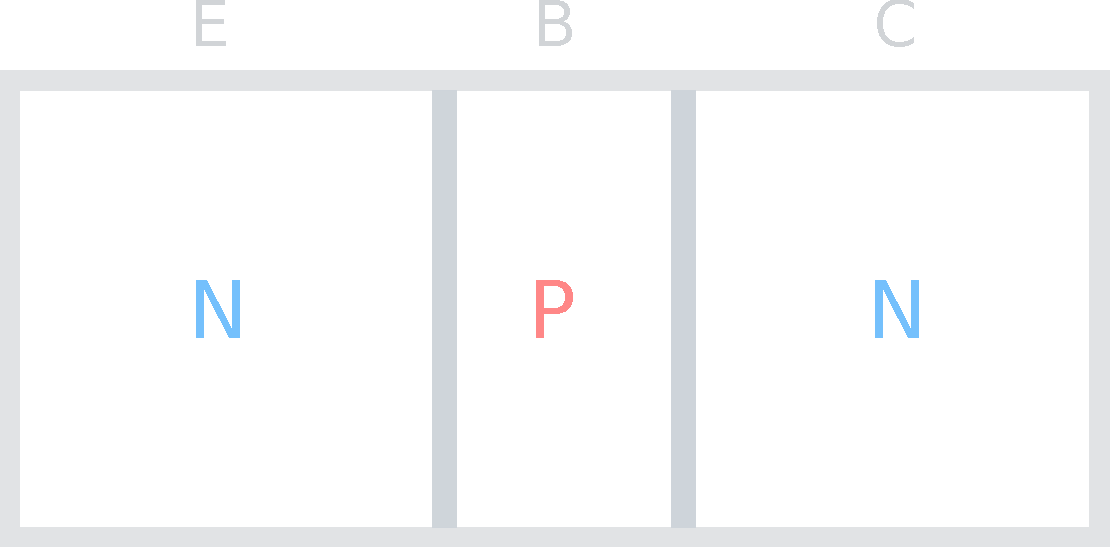
\includegraphics[width=0.618\textwidth]{1_1/npn.pdf}
  \end{center}
\end{figure}

Die Funktion des \emph{Bi}polartransistors basiert auf beiden Ladungsträger
-bzw. Halbleiterdotierungsarten. Je nach Transistortyp haben die drei Halbleitergebiete des Bipolartransistors die Dotierfolge NPN oder PNP, die einzelnen Regionen heißen Basis (B), Kollektor (C) und Emitter, welche unterschiedlich dotiert sind.\\

\begin{figure}[H]
\begin{center}
  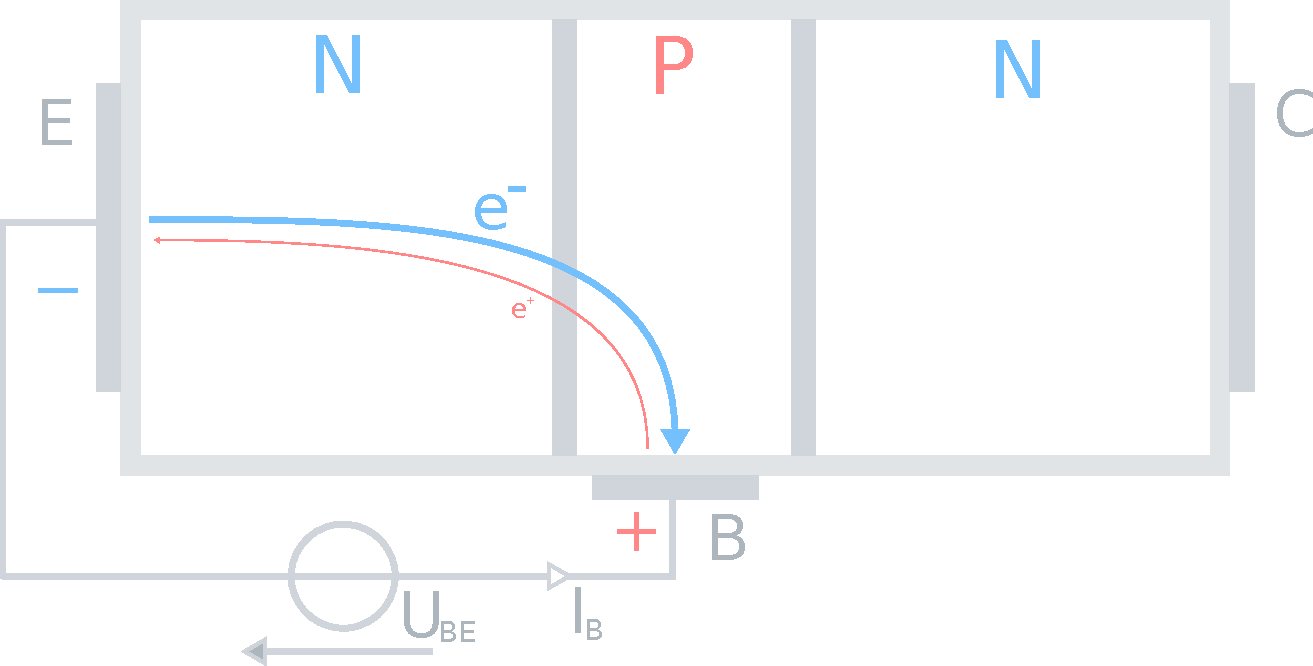
\includegraphics[width=0.618\textwidth]{1_1/npn_voltage.pdf}
  \end{center}
\end{figure}
Funktion am Beispiel des NPN-Transistors:
Ist die von außen anliegende Spannung $U_{\textrm{BE}}= 0\, \si{\volt}$, sind alle pn-Übergänge in Sperrrichtung und es fließt kein Strom durch den Transistor. Bei einer Spannung von etwa $U_{\textrm{BE}}=0.7\,\si{\volt}$ gerät der Basis-Emitter-Übergang in Durchlassrichtung. Löcher aus dem p-Gebiet (Basis) diffundieren in das n-Gebiet (Emitter) (vgl. Diode) und rekombinieren mit den dort befindlichen Leitungselektronen. Umgekehrt diffundieren die Elektronen des Emitters ebenfalls in die Basis. \\

\begin{figure}[H]
\begin{center}
  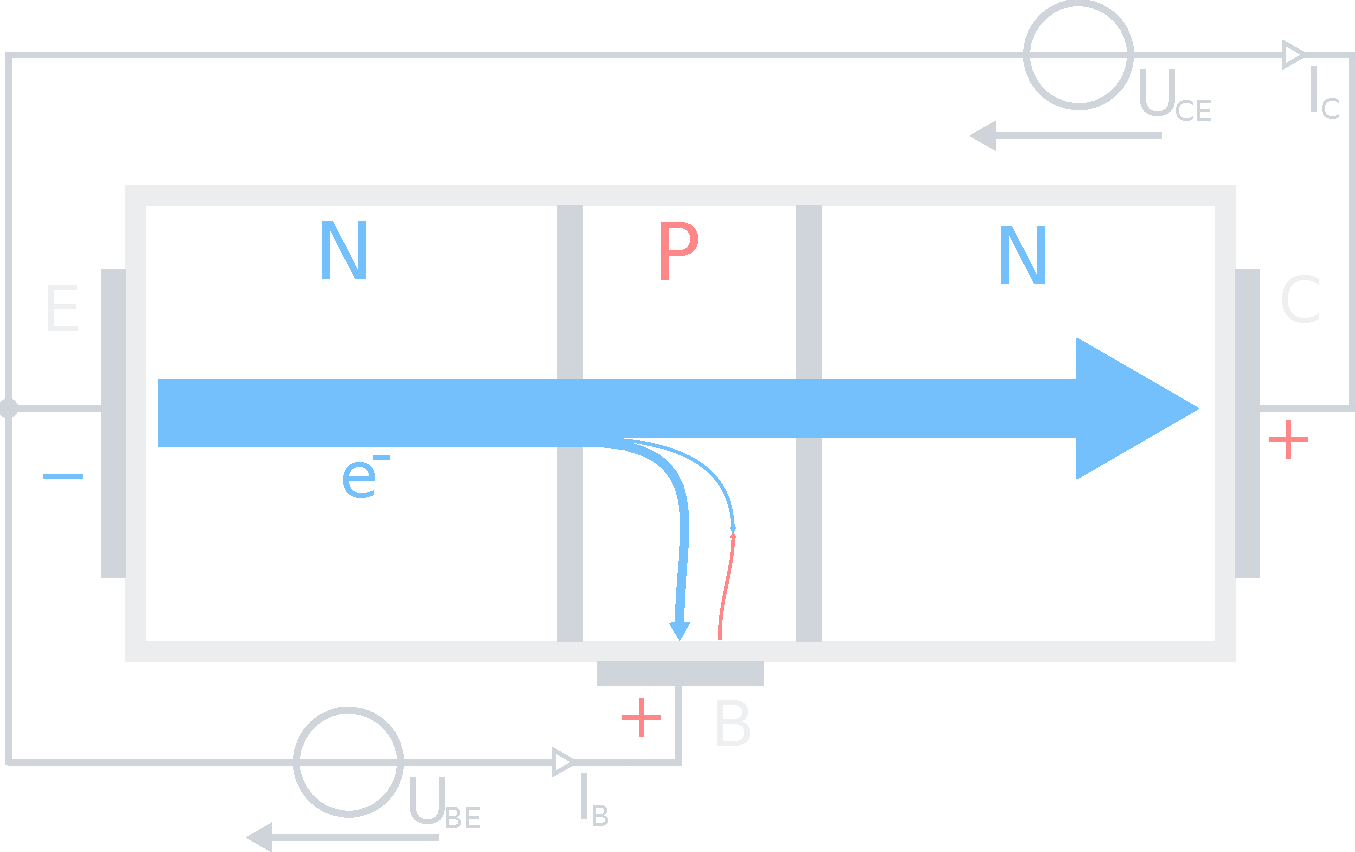
\includegraphics[width=0.618\textwidth]{1_1/npn_voltage_both.pdf}
  \end{center}
\end{figure}
Legt man eine zusätzliche Spannung an die Kollektor-Emitter-Strecke, so ist das elektrische Feld der Raumladungszone des Basis-Kollektorübergangs so gerichtet, dass sich die Elektronen des Emitters in Richtung Kollektor bewegen (Drift). Außerdem rekombinieren diese nicht in der Basis, da die Basisweite sehr gering ist. Es fließt ein Elektronenstrom zwischen Kollektor und Emitter, der durch einen deutlich geringeren Basisstrom gesteuert wird.


%%%%%%%%%% Ebers Moll
Ein mathematisches Modell zur Beschreibung des statischen Verhaltens des Bipolartransistors bietet das \emph{Ebers-Moll-Modell}:

\begin{center}
\begin{circuitikz}
  \draw (-1,0) to [short, o-, i<=$I_E$] (0,0);
  \draw (2,0) to [diode, v=$I_{ED}$] (0,0);
  \draw (2,0) to [diode, v^=$I_{CD}$] (4,0);
  \draw (4,0) to [short, -o, i<=$I_C$] (5,0);
  \draw (1.5,0) to [short] (2.5,0);
  \draw (2,0) to [short, *-o, i<^=$I_B$] (2,-2);
  \draw (0,0) to [short, *-] (0,2);
  \draw (2,0) to [short, *-*] (2,2);
  \draw (4,0) to [short, *-] (4,2);
  \draw (4,2) to [current source, l_=$A_N \cdot I_{ED}$, i=$$] (2,2);
  \draw (0,2) to [current source, l=$A_I \cdot I_{CD}$, i=$$] (2,2);
  \node[left] at (-1,0) {E};
  \node[right] at (5,0) {C};
  \node[below] at (2,-2) {B};
\end{circuitikz}
\end{center}

Knotengleichung am Emitter:

\[ I_E = I_{ED} - A_I \cdot I_{CD} \]
\[ I_E = I_{ES} \cdot \left( e^{\frac{U_{BE}}{U_T}} - 1 \right) - A_I \cdot I_{CS} \cdot \left( e^{\frac{U_{BC}}{U_T}} - 1 \right) \]

Knotengleichung am Kollektor:
\[ I_C = I_{CD} - A_N \cdot I_{CD} \]
\[ I_C = I_{CS} \cdot \left( e^{\frac{U_{BC}}{U_T}} - 1 \right) - A_N \cdot I_{ES} \cdot \left( e^{\frac{U_{BE}}{U_T}} - 1 \right) \]

Basis:
\[I_B = I_E - I_C\]
\[I_B = (1-A_N) \cdot I_{ES} \cdot \left( e^{\frac{U_{BE}}{U_T}} -1\right) - (1-A_I) \cdot I_{CS} \cdot \left( e^{\frac{U_{BC}}{U_T}} -1\right)\]


Im Normalbetrieb (Basis-Emitter-Übergang in Durchlass-, Basis-Kollektor-Übergang in Sperrrichtung) können die inversen Anteile des Modells vernachlässigt werden und es vereinfacht sich zu:
\begin{center}
\begin{circuitikz}
  \draw (-1,0) to [short, o-, i<=$I_E$] (0,0);
  \draw (2,0) to [diode, v=$I_{ED}$] (0,0);
  \draw (4,0) to [short, -o, i<=$I_C$] (5,0);
  \draw (2,0) to [short, *-o, i<^=$I_B$] (2,-2);
  \draw (2,0) to [short, -] (2,2);
  \draw (4,0) to [short, -] (4,2);
  \draw (4,2) to [current source, l_=$A_N \cdot I_{ED}$, i=$$] (2,2);
  \node[left] at (-1,0) {E};
  \node[right] at (5,0) {C};
  \node[below] at (2,-2) {B};
\end{circuitikz}
\end{center}
\[I_E = I_{ED}\] 
\[I_C = A_N \cdot I_{E}\] 
\[I_B = \frac{1-A_N}{A_N} \cdot I_{C}\] 



\subsection{Vierquadrantenkennlinienfeld}
\begin{figure}[H]
  \begin{center}
    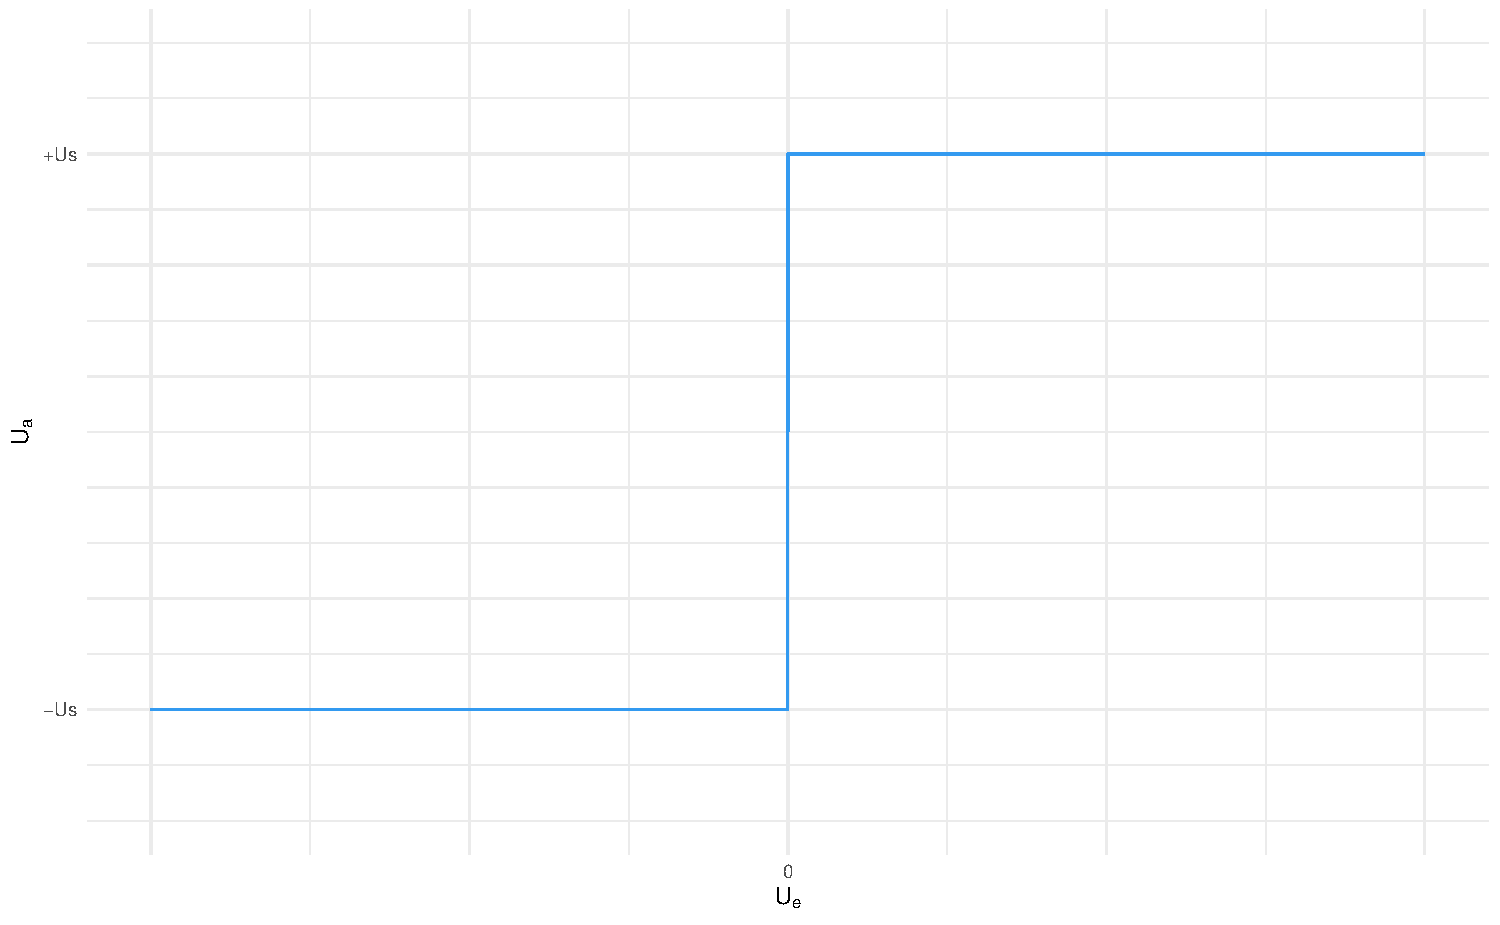
\includegraphics[width=0.618\textwidth]{1_2/opv_nofeed.pdf}
    \end{center}
    \caption{OPV-Kennlinie ohne Rückkopplung (ideal)}
 \end{figure}
\begin{figure}[H]
  \begin{center}
    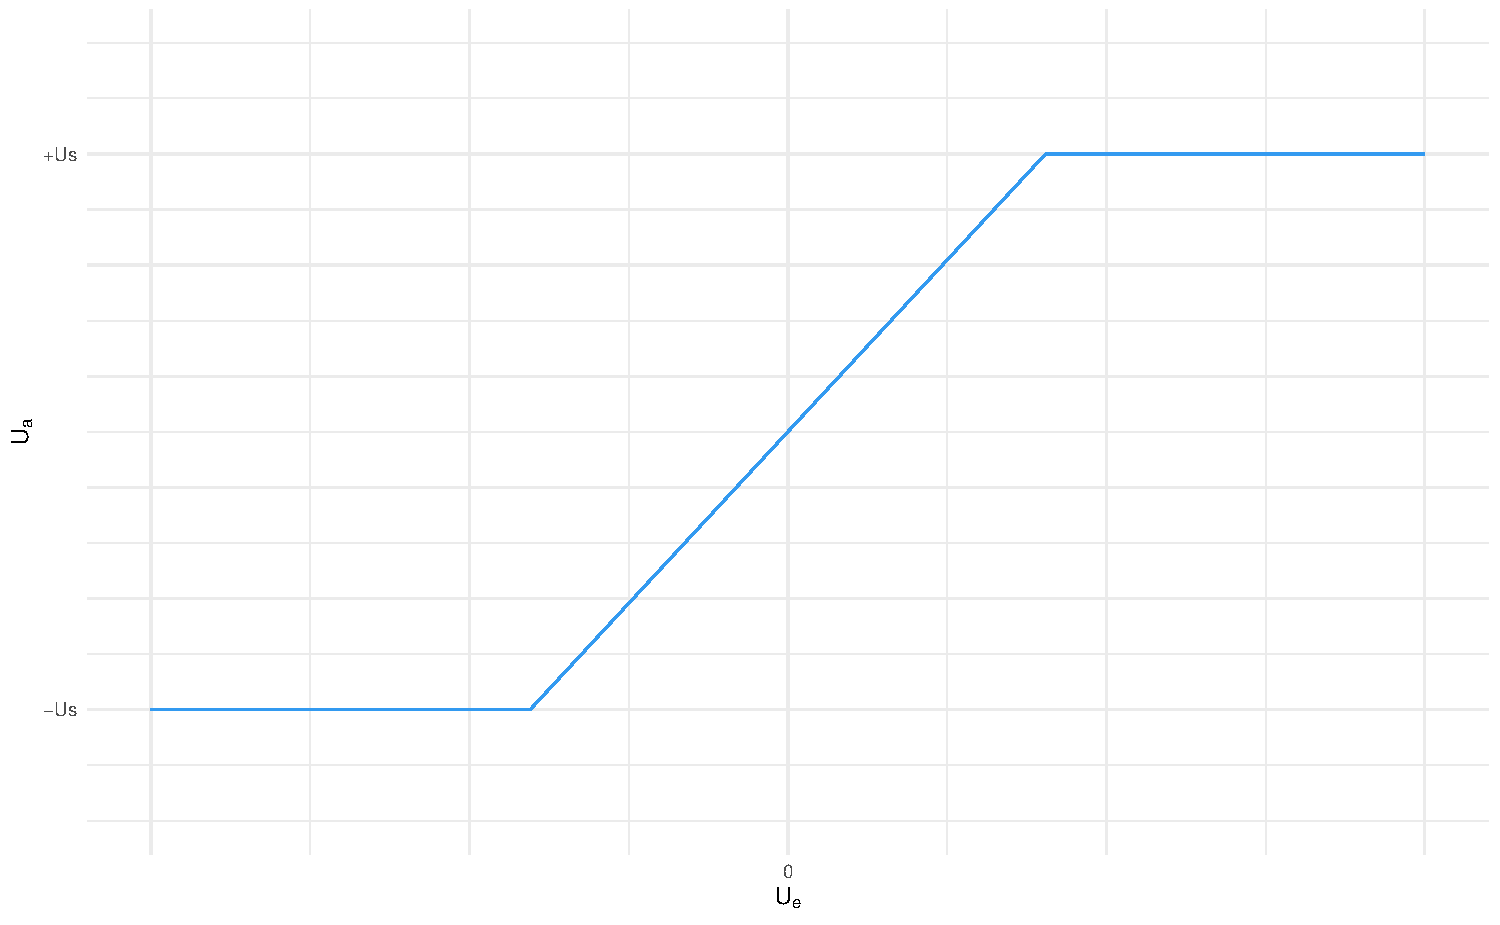
\includegraphics[width=0.618\textwidth]{1_2/opv_feed.pdf}
    \end{center}
    \caption{OPV-Kennlinie mit Rückkopplung}
 \end{figure}

Durch Rückführung eines Teils des Ausgangs- auf das Eingangssignal durch ein
Rückkopplungsnetzwerk wird der Operationsverstärker in einen linearen
Arbeitsbereich gebracht, wodurch die Verstärkung nicht mehr den Wert der der Leerlaufverstärkung (Abb. 1), sondern einen kontrollierten Verstärkungswert (Abb. 2) annimmt.


\subsection{Vierpolersatzschaltbild}
\subsubsection{Analyse mit CMD}\label{A3.3.1}

\begin{figure}[H]
  \begin{center}
    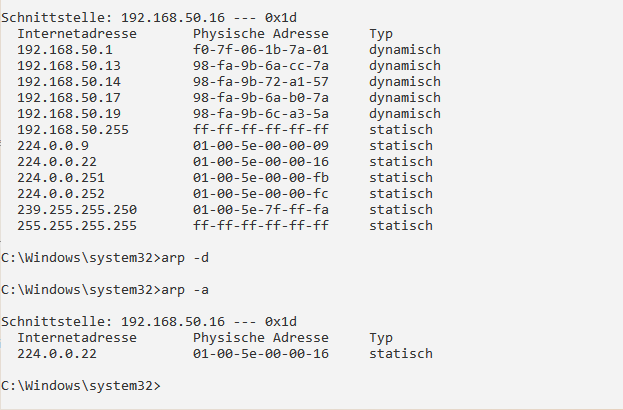
\includegraphics[width=0.618\textwidth]{graphics/versuch/3_3/arp_d}
    \caption{Löschen des ARP-Caches und folgendes Anzeigen der ARP-Tabelle}\label{abb_arp_d}
  \end{center}
\end{figure}

Im ersten Schritt wurde die ARP-Tabelle über die Eingabeaufforderung mithilfe von \inlinecode{arp -d} vollständig gelöscht (Abb. \ref{abb_arp_d}). Danach wurde der Nachbarrechner mit der IP-Adresse \inlinecode{192.168.50.14} mit dem \emph{ping}-Befehl angesprochen. Der Befehl hat den Zielrechner zuerst nach 4 Versuchen nicht erreicht, was daran lag, dass die Firewall am Ziel nicht deaktiviert war und den ping nicht durchgelassen hat. Nach Deaktivierung der Firewall lieferte der Befehl erfolgreiche Ergebnisse (Abb. \ref{abb_ping_1}).


\begin{figure}[H]
  \begin{center}
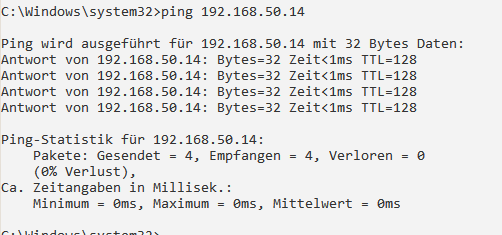
\includegraphics[width=0.618\textwidth]{graphics/versuch/3_3/ping_nach_abschalten_firewall_auf_zielrechner}
    \caption{Ping des Nachbarrechners 192.168.50.14}\label{abb_ping_1}
  \end{center}
\end{figure}

Nach dem ping-Befehl wurde erneut die ARP-Tabelle angezeigt (Abb \ref{abb_arp_neu}). Man kann erkennen, dass die IP-Adresse des Nachbarrechners in den Cache aufgenommen wurde. Außerdem wurde auch eine andere Adresse als Resultat des Empfangs einer ping-Nachricht aufgenommen, nämlich die \inlinecode{192.168.50.17}.

\begin{figure}[H]
  \begin{center}
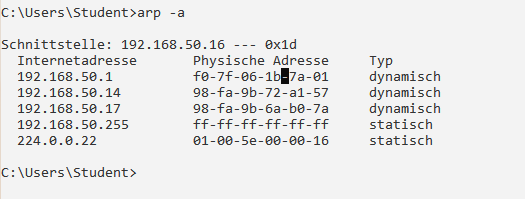
\includegraphics[width=0.618\textwidth]{graphics/versuch/3_3/arp_a_nach_ping_von_nachbar}
    \caption{ARP-Tabelleneinträge nach Ausführen des ping-Befehls}\label{abb_arp_neu}
  \end{center}
\end{figure}

Da der ping-Befehl, wie auch alle anderen Daten, durch Schicht 1 und 2 läuft, benötigt er die MAC-Adressen des Ziels, muss also die angegebene IP-Adresse übersetzen. Da die ARP-Tabelle gelöscht wurde, kann diese nicht zum Nachschlagen verwendet werden, weshalb ein ARP-Broadcast an alle Teilnehmer des Netzwerkes gesendet werden muss, um anzufragen, welche MAC-Adresse zum Host \inlinecode{192.168.50.14} gehört. Die notwendige Broadcast-Adresse ist wie in \ref{A3.2.2} ermittelbar, daher erscheint sie auch in Abb. \ref{abb_arp_neu}.\\

Die Multicast-Adresse \inlinecode{224.0.0.22} scheint fest eingebaut zu sein, da diese bereits in Abb. \ref{abb_arp_d} unmittelbar nach dem Löschen des ARP-Caches zu sehen war.

\subsubsection{Analyse mit Wireshark}
Mithilfe des Filters \inlinecode{arp || icmp} können nur die Pakete der für die Auswertung relevanten Protokolle betrachtet werden.\\


\begin{figure}[H]
  \begin{center}
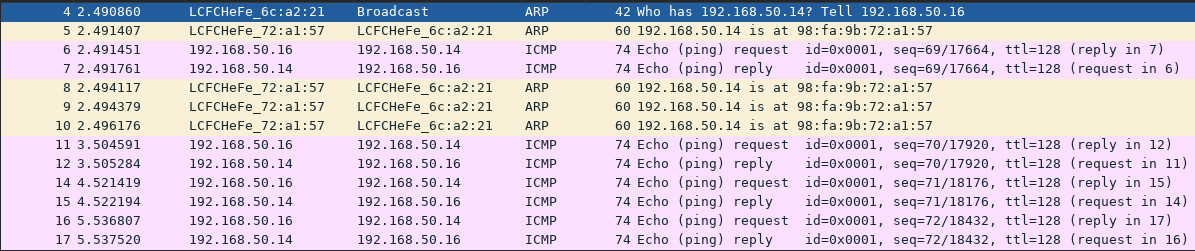
\includegraphics[width=\textwidth]{graphics/versuch/3_3/wireshark/allgemein}
    \caption{Gefilterte Ausgabe von Wireshark bei senden des ping-Kommandos}\label{wire_ping}
  \end{center}
\end{figure}

\paragraph{ARP}\label{A2.3.2.arp}
In Abb. \ref{wire_ping} erkennt man ersteinmal, dass genau 8 ICMP-Pakete aufgezeichnet wurden. Davon sind 4 Anfragen und 4 Antworten. Dies deckt sich mit Abb. \ref{abb_ping_1}, da der ping-Befehl genau 4 Mal gesendet wurde.\\

Vor Beginn des eigentlichen Pings findet man ein ARP-Paket. Hierbei handelt es sich um eine Broadcast-Nachricht zum Bestimmen der MAC-Adresse des Ziels. Dies ist notwendig, da vorher der ARP-Cache gelöscht wurde und sich dort kein Eintrag zur Ziel-IP-Adresse befindet (vgl. \ref{A3.3.1}).\\

Betachtet man die ARP-Anfrage genauer (Abb. \ref{arp_broadcast}), erkennt man im Ethernet-Frame, dass die Ziel-MAC-Adresse die bereits genannte \inlinecode{ff:ff:ff:ff:ff:ff} ist, welche für den Broadcast reserviert ist. Aus dem Quell-Feld erkennt man nun auch die Adresse der eigenen Netzwerkschnittstelle, nämlich \inlinecode{98:fa:9b:6c:a2:21}. Weiterhin ist im Header, wie zu erwarten, der Ethertype ARP, angegeben.

\begin{figure}[H]
  \begin{center}
    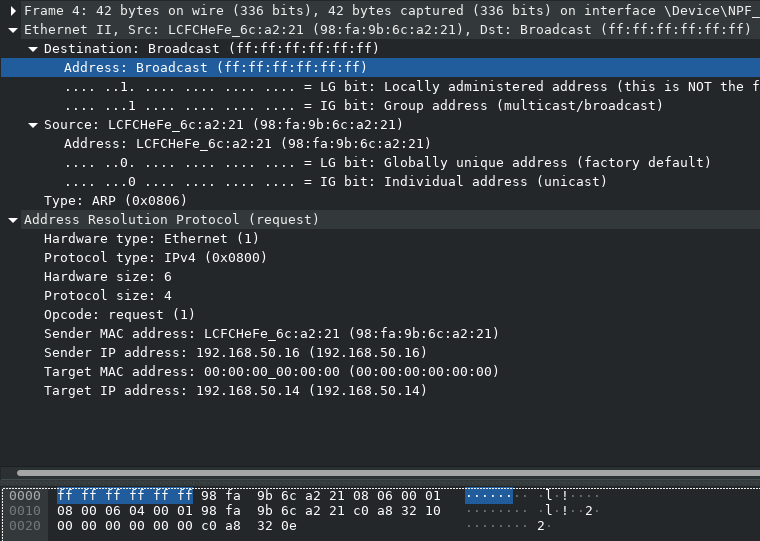
\includegraphics[width=\textwidth]{graphics/versuch/3_3/wireshark/arp_broadcast}
    \caption{Genauere Analyse der ersten ARP-Anfrage}\label{arp_broadcast}
  \end{center}
\end{figure}

Im folgenden Nutzdatenfeld befindet sich die ARP-Anfrage. Hier steht der Opcode 1 um zu signalisieren, dass es sich um eine Anfrage handelt. Außerdem enthält es Sender-MAC und -IP Adressen, sowie die bekannte Ziel-IP-Adresse. Das Feld Ziel-MAC-Adresse ist frei, da genau diese ja nachgefragt werden soll. Der angesprochene Host (sofern existent) sollte antworten und beide Felder ausfüllen. Dies geschieht dann auch in der zweiten Zeile von Abb. \ref{wire_ping}, in welcher die ARP-Antwort empfangen wurde.\\

Es antwortet also genau der Host auf den Broadcast mit einer ARP-Nachricht, dem die angefragte MAC-Adresse gehört. In Abb. \ref{arp_answer} ist der genaue Inhalt der ARP-Anwort dargestellt. Die Ziel-MAC ist nun nicht mehr der Broadcast, sondern die Adresse des Anfragers, die aus der Anfrage entnommen werden konnte. Mit dem Empfang dieser Daten ist das Ziel des ping-Befehls identifiziert.

\begin{figure}[H]
  \begin{center}
    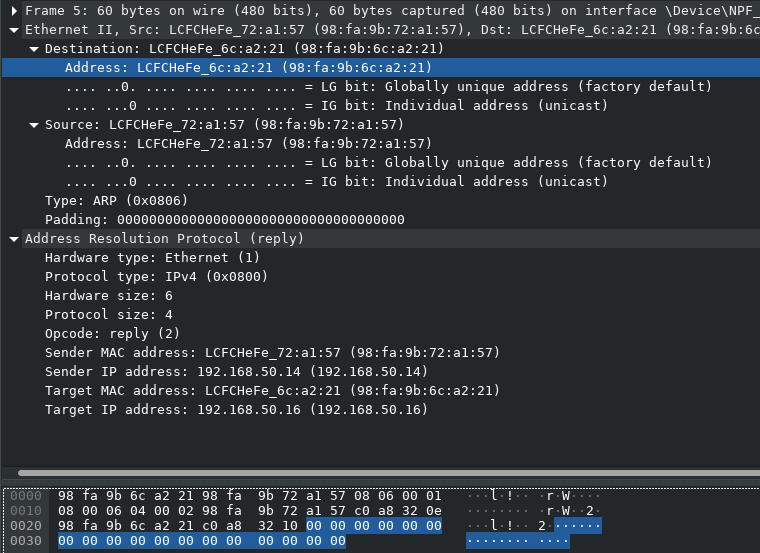
\includegraphics[width=\textwidth]{graphics/versuch/3_3/wireshark/arp_answer}
    \caption{Antwort auf die ARP-Anfrage}\label{arp_answer}
  \end{center}
\end{figure}

\label{CRC_erklar} Auffällig ist, dass in der Antwort aus Abb. \ref{arp_answer} im Ethernetframe zusätzlich ein 18-Byte langes Padding-Feld aus Nullen hinzugefügt wurde. Dies wird benötigt, um die minimale Länge des Frames von $64$ Byte zu erreichen. In Wireshark sind jedoch nur 60 Byte angezeigt, was daran liegt, dass das 4 Byte lange FCS-Feld zur Fehlererkennung mittels CRC automatisch weggelassen wird.\\

Dass die Framegröße in Abb. \ref{arp_broadcast} nur 42 und nicht 60 Byte lang ist, liegt daran, dass es sich um ein Paket handelt, das von der Schnittstelle gesendet wurde, die auch aufgezeichnet wird. In diesem Fall werden die Daten aufgezeichnet, bevor das Padding angefügt wird.\\

\paragraph{ICMP}
Da der ping-Befehl das ICMP-Protokoll verwendet, findet man dieses auch im Wireshark-Trace wieder, z.B. bei der ersten Anfrage (Abb. \ref{icmp_request}). Die allgemeine Struktur eines ICMP-Paketes ist in Abb. \ref{icmp_header} zu sehen.


\begin{figure}[H]
\centering
\resizebox{0.618\textwidth}{!}{\import{graphics/}{icmp_header.pdf_tex}}
\caption{Struktur des ICMP-Paketes}\label{icmp_header}
\end{figure}

Das Typ-Feld kann Werte von 0-255 annehmen und gibt die Art der Kontrollnachricht\footnote{\url{wikipedia.org/Internet_Control_Message_Protocol}} an. Beispielsweise bedeutet der Typ-Wert 0 eine Echo-Reply Nachricht (Echo Antwort, verwendet von ping) und der Wert 8 ein Echo-Request (Echo-Anfrage). Das Code-Feld gibt hierbei zusätzliche Informationen zum jeweiligen Typ-Feld. Bei den ICMP-Typen des ping-Befehls, also Echo-Reply und -Request ist der Inhalt des Code-Feldes 0.

\begin{figure}[H]
  \begin{center}
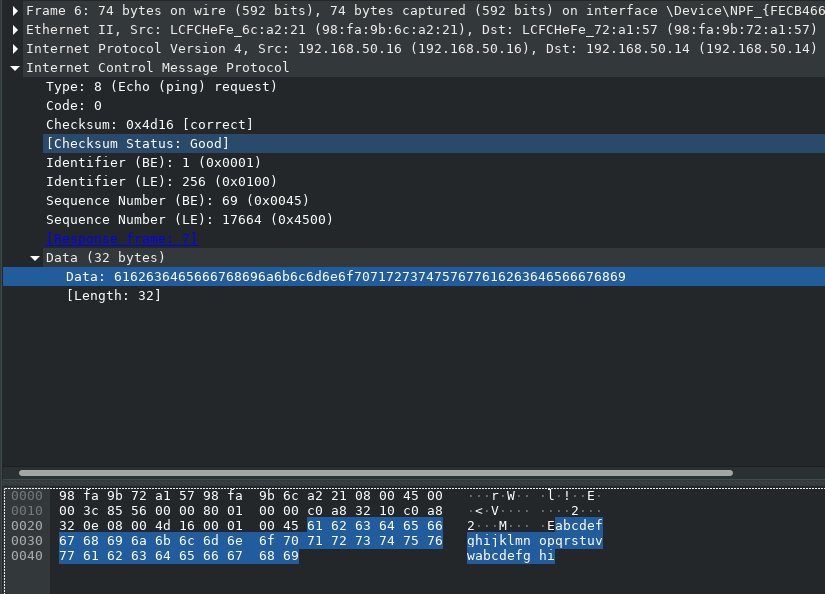
\includegraphics[width=\textwidth]{graphics/versuch/3_3/wireshark/ping_request}
    \caption{ICMP-Anfrage des ping-Befehls, Ausgabe von Wireshark mit geöffnetem ICMP-Paket}\label{icmp_request}
  \end{center}
\end{figure}

Auffällig ist hierbei zuerst, dass, im Gegensatz zum ARP-Beispiel, die ICMP-Daten in ein IP-Paket gepackt sind (Zeile 3 in Abb. \ref{icmp_request}). Das ist auch sinnvoll, da ICMP auf Ebene 3 agiert und eine konkrete Ziel-IP-Adresse benötigt, während ARP auf Ebene 2 mithilfe von Broadcasts arbeitet und somit nicht in Berührung mit dem IP-Header kommt.\\

Das ICMP-Paket in diesem Beispiel hat ein 32 Byte langes Datenfeld (max. ), welches mit 32 diversen ASCII-Zeichen gefüllt ist. Die Ausgabe der Eingabeaufforderung in Abb. \ref{abb_ping_1} bestätigt dies. Die Gesamtgröße des Paketes ist 40 Byte (abzählbar aus Wireshark-Ausgabe), die Header-Größe ist daher die Differenz, also 8 Byte, was auch mit der ICMP-Definition übereinstimmt.\\

Folgend kommt die ICMP-Antwort, wie sie in Abb. \ref{icmp_answer} zu sehen ist, vom erwarteten Host mit der  IP-Adresse \inlinecode{192.168.50.14}. Die Antwort enthält die gleichen Zeichen im ICMP-Datenfeld, nur das Typ-Feld wurde geändert von 8 (request) auf 0 (reply), was ebenfalls zu erwarten war.

\begin{figure}[H]
  \begin{center}
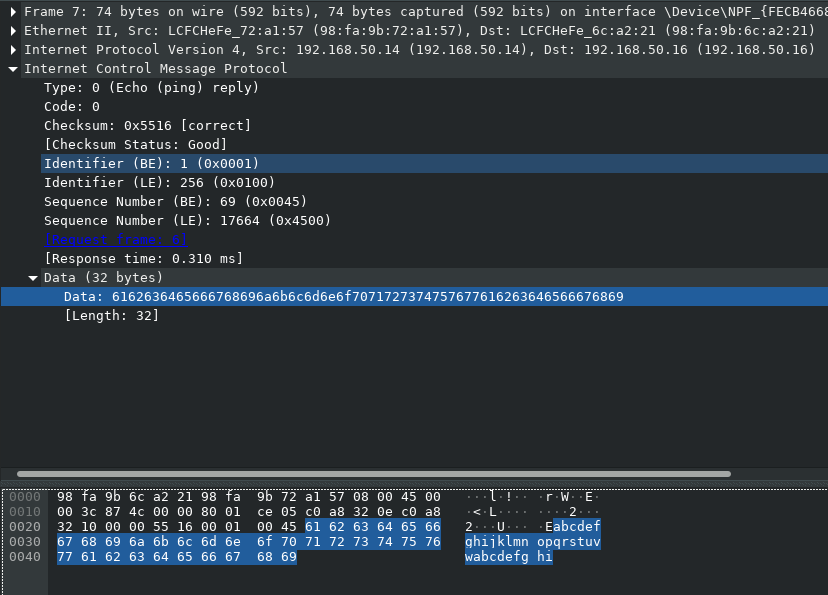
\includegraphics[width=\textwidth]{graphics/versuch/3_3/wireshark/ping_answer}
    \caption{ICMP-Antwort auf die Anfrage durch den ping-Befehl}\label{icmp_answer}
  \end{center}
\end{figure}

Der gesamte Ping-Prozess wird, wie bereits erwähnt, vier Mal wiederholt. Die dabei gesendeten bzw. empfangenen Pakete/Frames sind einschließlich des Datenfeldes äquivalent zu denen des ersten Pings, der hier behandelt wurde (nur Quell/Ziel-Adressen sind vertauscht).\\

Die Zeiten, die die CMD-Ausgabe des Befehls angibt, können ebenfalls in Wireshark bestätigt werden. In Abb. \ref{abb_ping_1} wird eine Zeit $<1\,\si{\milli\second}$ berichtet. Aus der Zeitdifferenz in Wireshark ergeben sich $310 \,\si{\micro\second}$.\\

In Abb. \ref{wire_ping} erkennt man 3 weitere ARP-Antworten vom Host \inlinecode{192.168.50.14}, obwohl nur eine Anfrage gestellt wurde. Die Antworten sind der bereits empfangenen ersten Antwort identisch. Weshalb genau diese erscheinen, konnte nicht geklärt werden.\\

\subsubsection{Flussdiagramm der Ping-Kommunikation}


\begin{figure}[H]
\centering
    \resizebox{\textwidth}{!}{\import{graphics/}{ping_flowchart.pdf_tex}}
    \caption{Flussdiagramm der Ping-Kommunikation}
\end{figure}

Das Flussdiagramm stellt den zeitlichen Ablauf der Kommunikation zwischen Sender (\inlinecode{192.168.50.16}) und Empfänger (\inlinecode{192.168.50.16}) dar. Für Sender und Empfänger sind jeweils die IP-Adressen als Endpunkt angegeben, allerdings sind diese nur für das Verständis, da nicht jedes Protokoll (wie z.B. ARP) diese zur Adressierung benötigt. Die Zeitangaben sind jeweils als sogenannte \glqq Delta Zeit\grqq, also der Zeitdifferenz zum vorherigen Ereignis dargestellt (Laufzeit, Wireshark $\rightarrow$ Einstellungen $\rightarrow$ Columns $\rightarrow$ delta Time).\\

Der Einfachheit halber wurden im Flussdiagramm nicht alle Felder der jeweiligen Pakete, sondern nur die für das Verständis der Kommunikation notwendigen dargestellt.

\subsubsection{ping-Overhead}
Für die Betrachtung des prozentualen Overheads wird das gesamte ICMP-Paket, so wie es der IP-Header umfasst, betrachtet. Wie vorher bereits bestimmt, beträgt die Größe dieses Paketes $32 \, \si{\byte} + 8 \, \si{\byte} = 40$ Byte. Der gesamte Frame, so wie er in das Netzwerk übertragen wird, beträgt laut Wireshark $74 \, \si{\byte}$ zu denen noch $4 \, \si{\byte}$ für das Ethernet-FCS Feld hinzukommen (siehe \ref{CRC_erklar}/ARP). Somit sind es $74 + 4 - 32 = 46$ Byte an Overhead. Der Prozentuale Overhead $o$ des ping-Befehls (genauer: des Standard-ping-Befehls unter Windows) ist demnach
\[o = \frac{46 \, \si{\byte}}{78 \, \si{\byte}} \cdot 100 \, \si{\percent} \approx 59 \, \si{\percent}\,.\]


\subsection{Transistorgrundschaltungen}
Die drei Grundschaltungen des Transistors werden nach dem der Ausgangs- und
Eingangsspannung gemeinsamen Potential benannt. Demnach existieren Emitter-,
Kollektor- und Basisschaltung. Zum Entfernen der Gleichanteile des Ein- und
Ausgangssignals werden Kondensatoren vor die Eingänge geschaltet, welche so
dimensioniert sind, dass sie für die Wechselanteile der Signale einen
Kurzschluss darstellen.

Bei der Arbeitspunkteinstellung werden die Kondensatoren entfernt und die
Widerstände im gewünschten Arbeitspunkt ($I_C, U_{CE}$) ermittelt.

\subsubsection{Emitterschaltung}

\begin{figure}[H]
  \begin{center}
    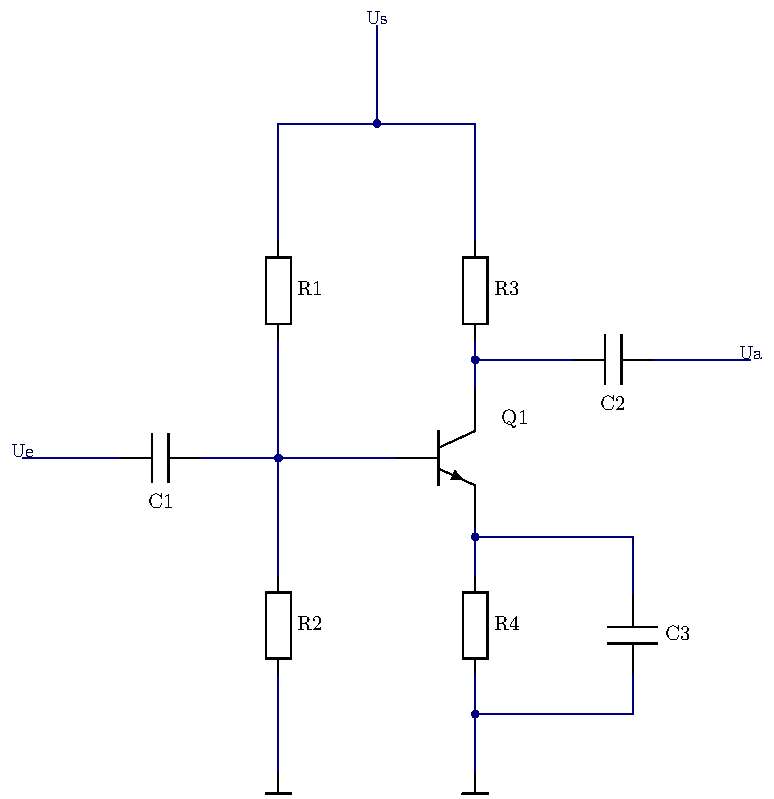
\includegraphics[width=0.618\textwidth]{circuits/commonEmitter.pdf}
  \end{center}
  \caption{Emitterschaltung}
\end{figure}

Mithilfe der Stromgegenkopplung durch den Widerstand $R_4$ lässt sich der
Arbeitspunkt gegenüber Änderungen der Stromverstärkung stabilisieren, er
verringert jedoch die Verstärkung und erhöht den Eingangs- und Ausgangswiderstand.
Man kann einen Kondensator ($C_3$) parallel schalten, um die negative Auswirkung
des Widerstands für Wechselsignale zu unterdrücken. Allgemein besitzt die
Emitterschaltung eine hohe Spannungsverstärkung sowie einen hohen Ein- und
Ausgangswiderstand.

\subsubsection{Kollektorschaltung (Emitterfolger)}
\begin{figure}[H]
  \begin{center}
    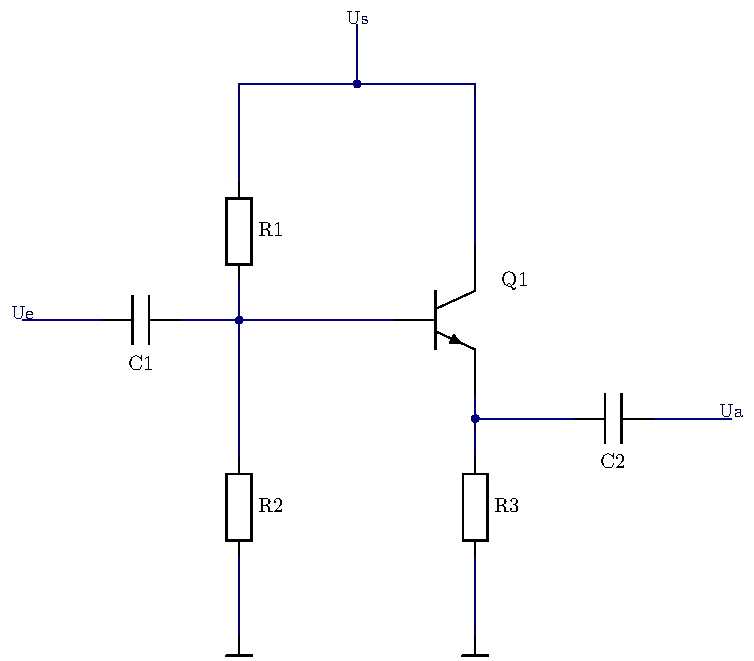
\includegraphics[width=0.618\textwidth]{circuits/commonCollector.pdf}
  \end{center}
  \caption{Kollektorschaltung}
\end{figure}

Das Ausgangsspannungssignal der Kollektorschaltung folgt etwa dem Eingangssignal
($-0.7\,\si{\volt}$), die Spannungsverstärkung ist $1$, der Ausgangsstrom ist
jedoch deutlich höher als der Eingangsstrom. Der Eingangswiderstand
der Schaltung ist daher sehr hoch, der Ausgangswiderstand ist umgekehrt proportional
der Steilheit des Transistors, also in der Regel sehr gering, weshalb sich die
Schaltung gut als Impedanzwandler eignet. 

Die Arbeitspunkteinstellung ist analog der Arbeitspunkteinstellung bei der Emitterschaltung.
Zusätzlich kann, wie bei der Emitterschaltung, ein Kollektorwiderstand
eingeführt werden, welcher dann über einen, ebenfalls zusätzlichen, vom
Kollektor an Masse
geführten Kondensator wechselspannungsmäßig kurzgeschlossen wird.

\[R_{ein} \approx r_\pi (1 + g_m \cdot R_3)\]
\[R_{aus} \approx \frac{1}{g_m}\]

\subsubsection{Basisschaltung}
\begin{figure}[H]
  \begin{center}
    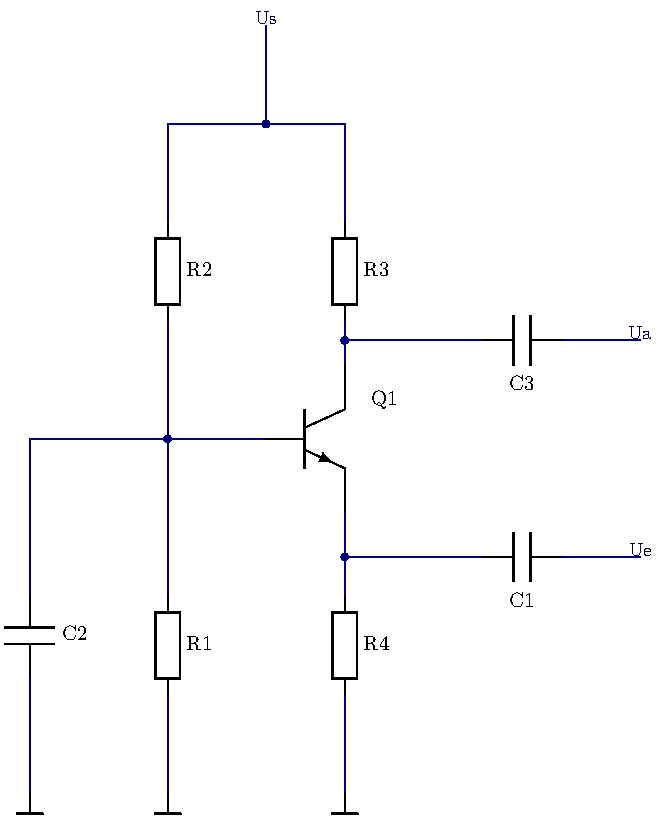
\includegraphics[width=0.618\textwidth]{circuits/commonBase.pdf}
  \end{center}
  \caption{Basisschaltung}
\end{figure}

Die Basisschaltung kennzeichnet sich durch einen sehr geringen
Eingangswiderstand, einen hohen Ausgangswiderstand sowie eine hohe Spannungsverstärkung.
Auch hier geschieht die Arbeitspunkteinstellung über das 4-Widerstandsnetzwerk
aus $R_2, R_1, R_3$ und $R_4$. Der Kondensator $C_2$ schließt im
Kleinsignalersatzschaltbild die Widerstände $R_1$ und $R_2$ kurz und bringt die Transistorbasis auf Massepotential.
\[R_{ein} \approx \frac{1}{g_m}\]
\[R_{aus} \approx r_0 \]

\subsection{Dimensionierung einer Emitterstufe}
Die Spannung über dem Emitterwiderstand $U_{R_4}$ wird gewählt
\[ U_{R_4} = 1 \, \si{\volt}\]

\noindent Damit ergibt sich die Spannung $U'$ am Basisspannungsteiler zu
\[ U' = 1 \, \si{\volt} + 0.7 \, \si{\volt} = 1.7 \, \si{\volt}\]

Der Querstrom durch den Spannungsteiler wird so hoch gewählt, dass dieser
bezüglich des Basisstroms als unbelastet angesehen werden kann. 
\[I_{R_1} = 8 \cdot I_B\]

\noindent Der Basisstrom
\[I_B = \frac{I_C}{\beta} = \frac{4.5 \, \si{\milli\ampere}}{158} = 27.22 \, \si{\micro\ampere}\]

\noindent führt zu den Widerstandswerten des Basisspannungsteilers
\[R_2 = \frac{U'}{8 \cdot I_B} = \frac{1.7 \, \si{\volt}}{8 \cdot 27.22 \,
    \si{\micro\ampere}} = 7.87 \, \si{\kilo\ohm}\]

\[R_1 = \frac{U_s - U'}{9 \cdot I_B} = \frac{10.3 \, \si{\volt}}{244.98 \,
    \si{\micro\ampere}} = 42.2 \, \si{\kilo\ohm}\]

Die verbleibenden Widerstände sind
\[ R_4 =  \frac{U_{R_4}}{I_{C,A}} = \frac{1 \, \si{\volt}}{4.3 \,
    \si{\milli\ampere}} = 232 \, \si{\ohm}\]

\[R_3 = \frac{U_s - U_{R_4} - U_{CE,A}}{I_{C,A}} = \frac{5 \, \si{\volt}}{4.3 \,
  \si{\milli\ampere}} = 1.15 \, \si{\kilo\ohm}\]

Die Widerstandswerte wurden so gerundet, dass sie jeweils in eine E-Reihe passen.

Der Kondensator parallel zu $R_3$ kann so gewählt werden, dass seine Reaktanz $X_C$ bei der
niedrigsten Signalfrequenz gleich $1/10\, R_3$ ist.

\subsection{Temperaturabhängigkeiten}
\begin{figure}[H]
  \begin{center}
    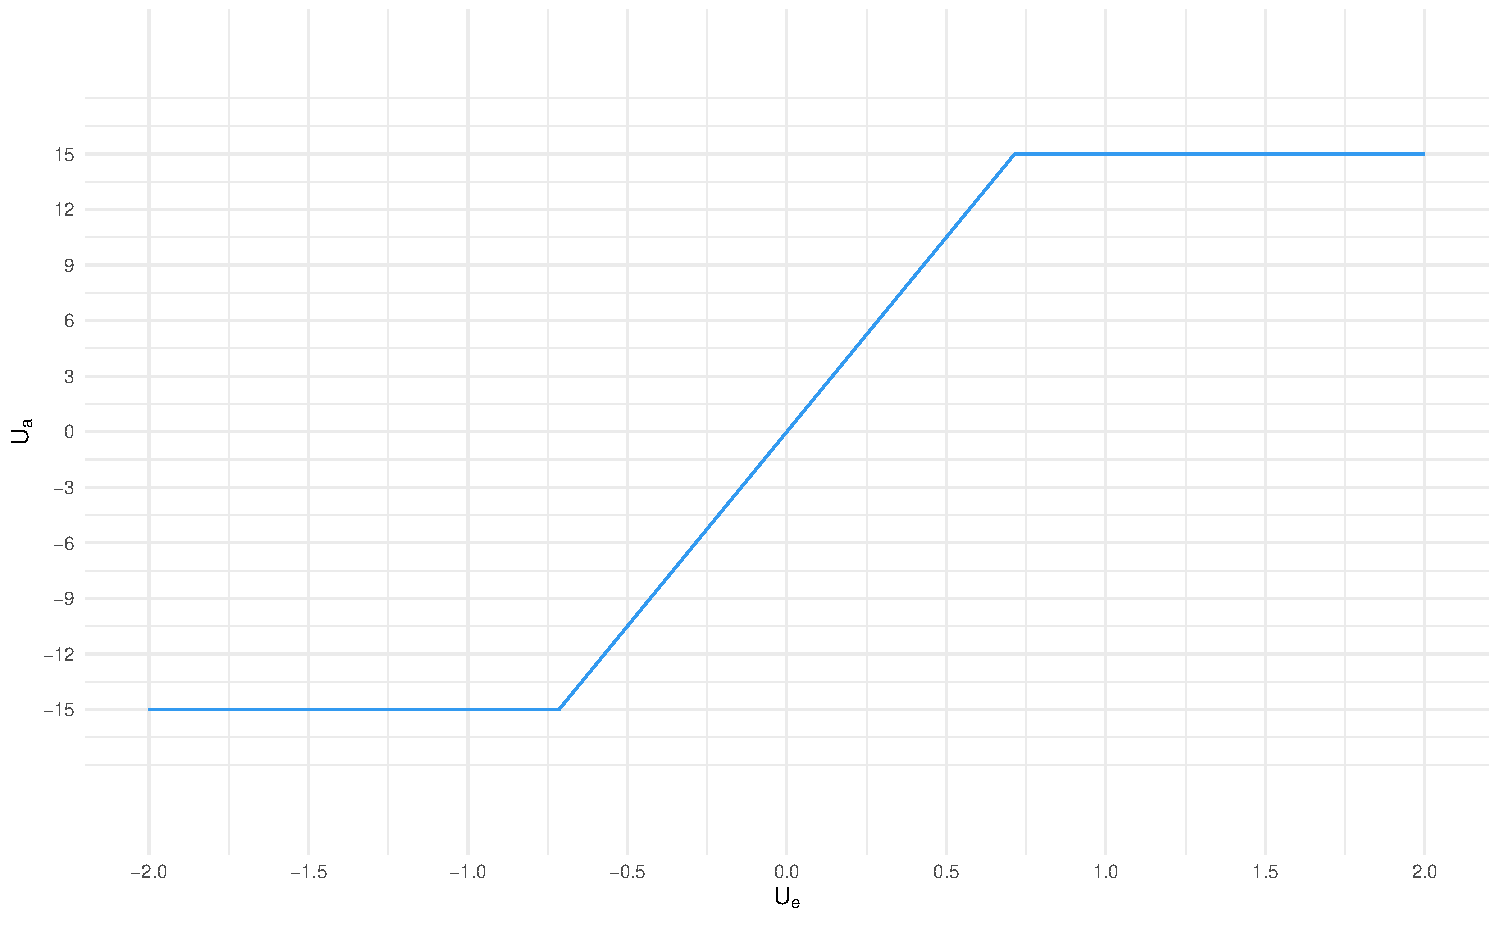
\includegraphics[height=0.618\textwidth]{1_6/opv_nichtinv_verst.pdf}
    \end{center}
    \caption{Kennlinie einer nichtinvertierenden OPV-Schaltung mit einer
      Verstärkung von $V_u = 21$ und einer Versorgungsspannung von $U_s = \pm 15
      \, \si{\volt}$}
 \end{figure}

\subsection{Bestimmung der Grundschaltungsparameter}
Die Parameter werden nach dem physikalischen Ersatzschaltbild des
Bipolartransistors ohne parasitäre Kapazitäten bestimmt. Bei der
Kleinsignalanalyse werden alle Kapazitäten sowie Spannungsquellen als
Kurzschlüsse behandelt.

\subsubsection{Emitterschaltung}

\begin{figure}[H]
  \begin{center}
    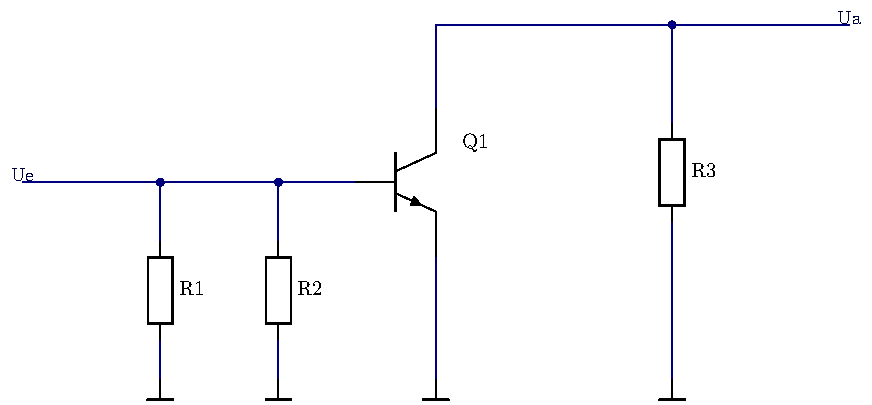
\includegraphics[width=0.618\textwidth]{circuits/commonEmitter_ESB1.pdf}
  \end{center}
  \caption{Kleinsignalersatzschaltbild der Emitterschaltung (Abb. 3)}
\end{figure}

\begin{figure}[H]
  \begin{center}
    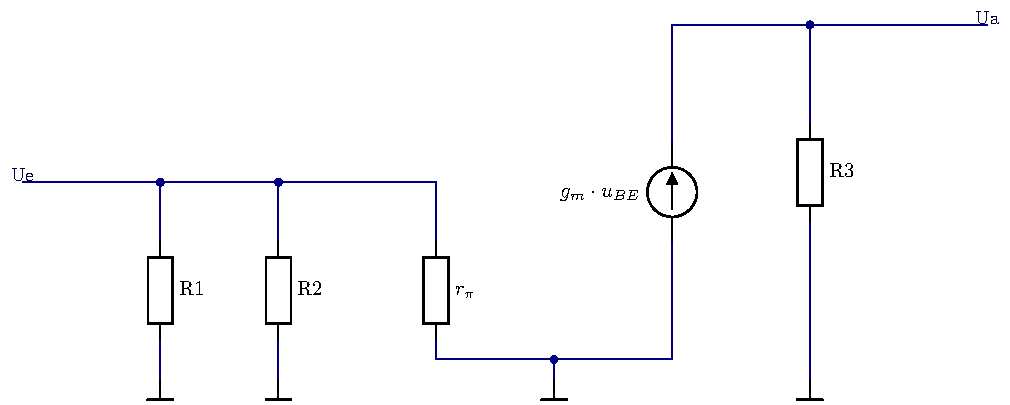
\includegraphics[width=0.618\textwidth]{circuits/commonEmitter_ESB2.pdf}
  \end{center}
  \caption{ESB Abb. 6, Transistor durch phys. ESB ersetzt}
\end{figure}

\noindent Eingangswiderstand:
\[r_e = \frac{U_e}{I_e} = R_1 // R_2 // r_\pi\]
\noindent Ausgangswiderstand:
\[r_a = \frac{U_a}{I_a} = r_0 // R_3 \]
\noindent Spannungsverstärkung:
\[V_u = \frac{U_2}{U_1}\]

\begin{gather*}
  U_2 = g_m \cdot u_{BE} \cdot (r_0 // R_3) = g_m \cdot U_1 \cdot (r_0 // R_3)\\
  V_u = g_m \cdot (r_0 // R_3)
\end{gather*}

\noindent Stromverstärkung:
\[V_i = \frac{I_2}{I_1}\]
\[I_1 = \frac{U_1}{r_\pi} + U_1 (\frac{1}{R_2} + \frac{1}{R_1})\]
\[I_B = \frac{U_1}{r_\pi} = I_1 - U_1 (\frac{1}{R_2} + \frac{1}{R_1})\]
\[I_2 = g_m \cdot U_1 \rightarrow U_1 = \frac{I_2}{g_m}\]
\[ \frac{I_2}{g_m \cdot r_\pi}  = I_1 - \frac{I_2}{g_m} (\frac{1}{R_2} + \frac{1}{R_1}) \]
\[ \frac{1}{g_m \cdot r_\pi}  = \frac{I_1}{I_2} - \frac{1}{g_m} (\frac{1}{R_2} + \frac{1}{R_1}) \]
\[\frac{I_2}{I_1} = V_i = \frac{1}{ \frac{1}{g_m} (\frac{1}{r_\pi} +
    \frac{1}{R_2} + \frac{1}{R_1}) }\]

\noindent Leistungsverstärkung:
\[V_p = \frac{P_2}{P_1} = \frac{U_2 \cdot I_2}{U_1 \cdot I_1} = V_u \cdot V_i\]
\[V_p = \frac{g_m^2 \cdot (r_0 // R_3)}{\frac{1}{r_{\pi}} + \frac{1}{R_2} + \frac{1}{R_1}}\]

%%%%%%%%%%%%%%%%%%%%%%%%%%%%%%%%%%%%%%%%%
\subsubsection{Kollektorschaltung}
\begin{figure}[H]
  \begin{center}
    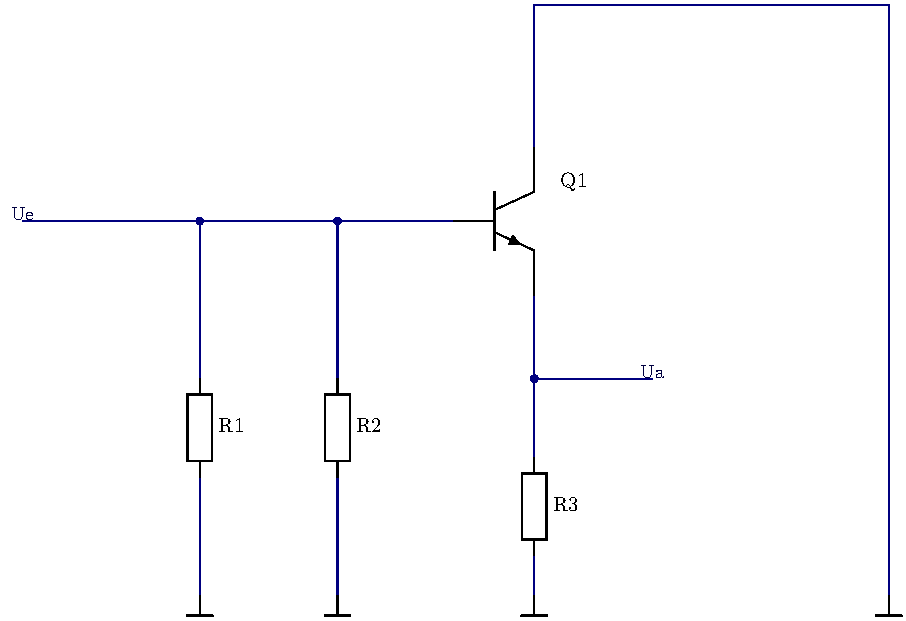
\includegraphics[width=0.618\textwidth]{circuits/commonCollector_ESB1.pdf}
  \end{center}
  \caption{Kleinsignalersatzschaltbild der Kollektorschaltung (Abb. 4)}
\end{figure}


\begin{figure}[H]
  \begin{center}
   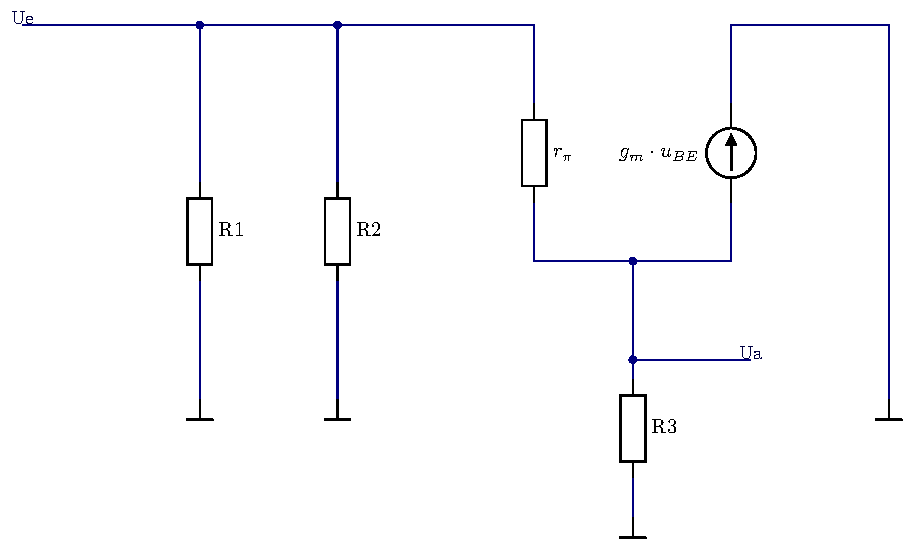
\includegraphics[width=0.618\textwidth]{circuits/commonCollector_ESB2.pdf}
  \end{center}
  \caption{ESB Abb. 8, Transistor durch phys. ESB ersetzt}
\end{figure}
\noindent Eingangswiderstand
\[ r_e = \frac{U_1}{I_1}\]
\[ r_e = R_1 // R_2 // (r_\pi + \beta_N R_3)\]

\noindent Ausgangswiderstand
\[ r_a = \frac{U_2}{I_2}|_{U_1 = 0}\]
\[U_2 = U_{BE}\]
\[r_a = R_3 // \frac{r_\pi }{\beta_N + 1}\]
\[r_a \approx \frac{1}{g_m}\]

\noindent Spannungsverstärkung
\[ V_u = \frac{U_2}{U_1}\]
\[V_u = \frac{1}{1+ \dfrac{1}{g_m \cdot R_3}} \approx 1\]

%%%%%%%%%%%%%%%%%%%%%%%%%%%%%%%%%%%%%%%%%
\subsubsection{Basisschaltung}
\begin{figure}[H]
  \begin{center}
    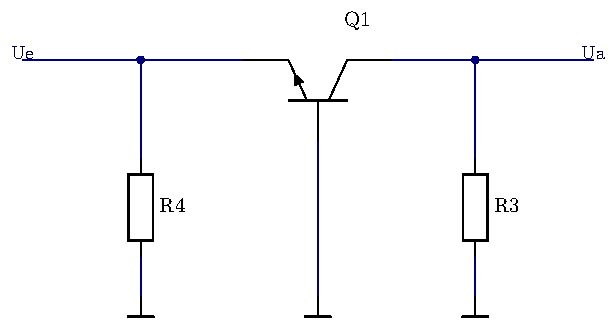
\includegraphics[width=0.618\textwidth]{circuits/commonBase_ESB1.pdf}
  \end{center}
  \caption{Kleinsignalersatzschaltbild der Basisschaltung (Abb. 5)}
\end{figure}

\begin{figure}[H]
  \begin{center}
    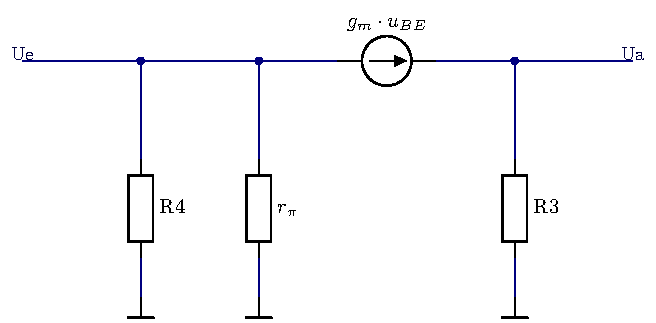
\includegraphics[width=0.618\textwidth]{circuits/commonBase_ESB2.pdf}
  \end{center}
  \caption{ESB Abb. 10, Transistor durch phys. ESB ersetzt}
\end{figure}

\noindent Eingangswiderstand
\[ r_e = \frac{U_1}{I_1}\]
\[0 = I_1 + \frac{U_1}{R_4} + \frac{U_1}{r_\pi} + g_m U_{BE} \]
\[I_1 = - \frac{U_1}{R_4} - \frac{U_{BE}}{r_\pi} - g_m U_{BE} \]
\[U_{BE} = - U_1\]
\[I_1 = \frac{U_1}{R_4} + \frac{U_1}{r_\pi} + g_m U_{1} \]
\[ \frac{I_1}{U_1} = \frac{1}{R_4} + \frac{1}{r_\pi} + g_m \]
\[ r_e = \frac{1}{ \frac{1}{R_4} + \frac{1}{r_\pi} + g_m} \]
\[g_m = \frac{B_n}{r_\pi}\]
\[ r_e = \frac{1}{\frac{1}{R_4} + \frac{1}{r_\pi} (1+B_N)} \]
\[ r_e = \frac{1}{R_4} // (r_\pi (\frac{1}{1+B_N}))\]

\noindent Ausgangswiderstand
\[ r_a = \frac{U_2}{I_2}|_{U_e = 0}\]
\[ I_2 = g_m U_{BE} + \frac{U_2}{R_3 // r_0}\]
\[ U_{BE} = 0\]
\[ r_a = R_3 // r_0\]

\noindent Spannungsverstärkung
\[V_u = \frac{U_2}{U_1}\]
\[U_2 = -g_m \cdot U_{BE} (R_3 // r_0)\]
\[U_{BE} = - U_{1}\]
\[ \frac{U_2}{U_1} = V_u = g_m (R_3 // r_0)\]

\subsection{Messtechnische Bestimmung der Ein- und Ausgangsparameter}
\subsubsection{Bestimmung des Eingangswiderstands}
Allgemein gelingt die Widerstandsmessung indirekt durch eine Spannungs- und
Strommessung und anschließende Division der gemessenen Größen. 

\subsubsection{Bestimmung des Ausgangswiderstands}
Der Zusammenhang zwischen Lastwiderstand und Ausgangswiderstand des Verstärkers
ist linear (Zweipol)
\[R_a = \frac{U_{a,0} - U_{a,Last}}{I_{a,Last}}\]
\[R_a = \frac{U_{a,0} - U_{a,Last}}{U_{a,Last}} \cdot R_L\]
\[R_a = R_L \cdot \left(\frac{U_{a,0}}{U_{a,Last}}-1 \right)\]

Wobei $U_{a,0}$ die Leerlaufspannung am Ausgang, $U_{a,Last}$ die
Spannung am Ausgang bei Belastung mit dem Lastwiderstand $R_L$, und $R_a$ der
Ausgangswiderstand des Verstärkers ist.

Aus der Gleichung lässt sich erkennen, dass $R_a = R_L$ wenn $U_{a,Last} =
U_{a,0}/2$ ist. D.h. die Ausgangsspannung $U_{a,Last}$ kann bei
Belastung mit einem bekannten Lastwiderstandswert gemessen und anschließend in
der obigen Gleichung verwendet werden oder sie kann auf den halben Wert der
Leerlaufausgangsspannung durch einen variablen Lastwiderstand eingestellt
werden, wonach eine Messung des Lastwiderstandes folgt.


\subsubsection{Bestimmung der Verstärkungen}
Da die Verstärkungen frequenzabhängig sind und somit das Verhältnis von Ein- und
Ausgangsspannung (wechselspannungsmäßig) nicht konstant ist, muss man messtechnisch die
Übertragungsfunktion ermitteln, was beispielsweise durch das Durchlaufen mehrerer
Signalfrequenzen und anschließender Darstellung der
Ausgangsamplituden/-differenz erreicht werden kann (wobbeln). 

\subsection{Bootstrapschaltung}
\subsubsection{Differenzverstärker}

\begin{figure}[H]
  \begin{center}
    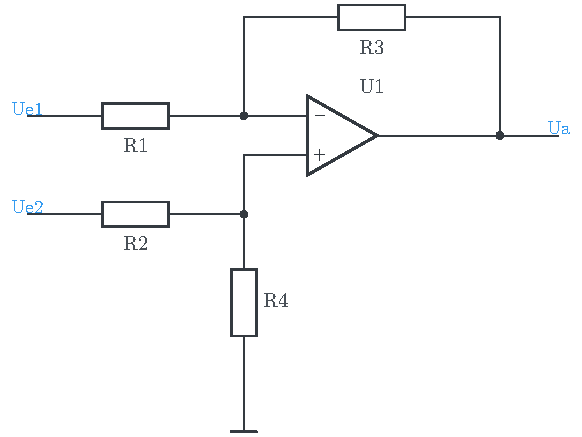
\includegraphics[width=0.618\textwidth]{circuits/differenz.pdf}
  \end{center}
  \caption{Differenzverstärkerschaltung}
\end{figure}

Der Differenzverstärker verstärkt die Differenz der Spannungen $U_{e1}$ und $U_{e2}$.

\begin{gather*}
  \intertext{Überlagerung:}
  U_a = U_a' + U_a''\\
  U_a' = U_a|_{U_{e2} = 0} = - U_{e1} \cdot \frac{R_3}{R_1}\\
  U_a'' = U_a|_{U_{e1} = 0} = U_p \cdot \left(1+\frac{R_3}{R_1}\right)\\
  = U_{e2}  \frac{R_4}{R_2 + R_4} \cdot \left(1+\frac{R_3}{R_1}\right)\\
  U_a = U_{e2}  \cdot \frac{R_4}{R_2 + R_4} \cdot \left(1+\frac{R_3}{R_1}\right) -
  U_{e1} \cdot \frac{R_3}{R_1}\\
  U_a = U_{e2}  \cdot \frac{R_4}{R_2 + R_4} + U_{e2} \cdot \frac{R_4}{R_2 + R_4}
  \cdot \frac{R_3}{R_1} - U_{e1} \cdot \frac{R_3}{R_1}
\end{gather*}
\noindent Wenn gilt $\frac{R_3}{R_1} = \frac{R_4}{R_2}:$
\eqbox{
  U_a = \frac{R_3}{R_1}\left(U_{e2} - U_{e1}\right)
}{0.382\textwidth}

\noindent Wenn alle Widerstände gleich dimensioniert werden:
\eqbox{
  U_a = U_{e2} - U_{e1}
}{0.382\textwidth}


\subsubsection{Instrumentationsverstärker}

\begin{figure}[H]
  \begin{center}
    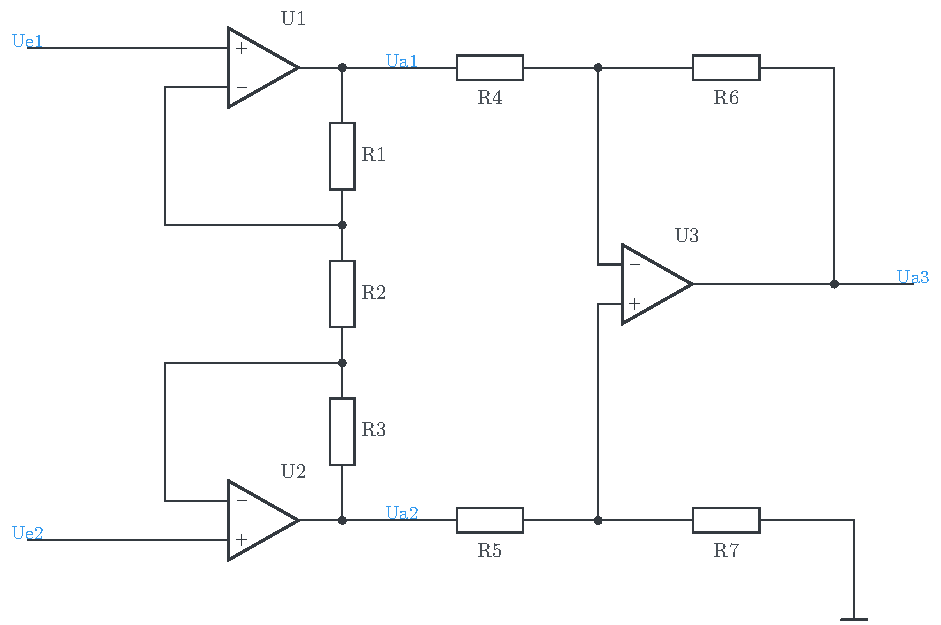
\includegraphics[height=0.618\textwidth]{circuits/instrument.pdf}
  \end{center}
  \caption{Instrumentationsverstärkerschaltung}
\end{figure}

\begin{gather*}
  \intertext{Virtuelle Masse, $U_d = 0$:}
  U_{R_2} = U_{e1} - U_{e2}\\
  I_{R_2} = \frac{U_{e1} - U_{e2}}{R_2}\\
  \intertext{für $I_n = 0$:}
  I_{R_1} = I_{R_2} = I_{R_3}\\
  U_{a1,2} = U_{a1} - U_{a2} = I_{R_3} (R_1 + R_2 + R_3)\\ 
  U_{a1} - U_{a2} = \frac{U_{e1}-U_{e2}}{R_2} (R_1 + R_2 + R_3)\\ 
  \intertext{für $R_1 = R_3$:}
  U_{a1} - U_{a2} = U_{e1} - U_{e2} \left( 1 + \frac{2 \cdot R_1}{R_2}\right)
\end{gather*}
  der Dritte OPV ist als Differenzverstärker geschaltet\\
  für $R_4 = R_5 = R_6 = R_7$ ist die Verstärkung $V_{OPV3} = -1$
    (Eingangsdifferenz tauschen)

\eqbox{
  U_{a3} = (U_{e2} - U_{e1}) \cdot (1 + \frac{2\cdot R_1}{R_2})
}{0.618\textwidth}
Die Verstärkung ist somit durch $R_2$ einstellbar
\subsubsection{Summierer}

\begin{figure}[H]
  \begin{center}
    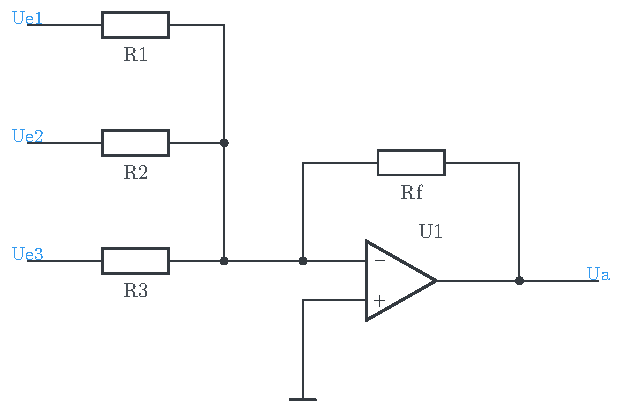
\includegraphics[width=0.618\textwidth]{circuits/summier.pdf}
  \end{center}
  \caption{Summierverstärkerschaltung}
\end{figure}

Der Summierverstärker verstärkt die Summe der gewichteten Eingangsspannungen.

\begin{gather*}
  I_{\mathrm{IN}} = \sum_{n=1}^N{I_{en}} = \frac{U_{e1}}{R_1}+
  \frac{U_{e2}}{R_2} + \cdots + \frac{U_{eN}}{R_N}\\
\end{gather*}
\eqbox{
  U_a = -\left( \frac{R_f}{R_1} U_{e1} + \frac{R_f}{R_2} U_{e2} + \cdots +
    \frac{R_f}{R_N} U_{eN} \right)
  }{0.618\textwidth+5mm}

\subsubsection{Integrator}
\begin{figure}[H]
  \begin{center}
    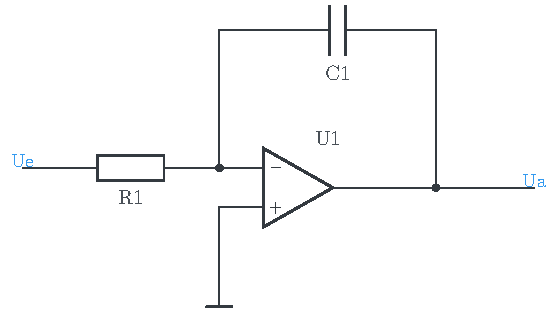
\includegraphics[width=0.618\textwidth]{circuits/integrier.pdf}
  \end{center}
  \caption{Integratorschaltung}
\end{figure}

\begin{gather*}
i_{R_1} = - i_{C_1}\\
\frac{u_e}{R_1} = - C_1 \cdot \frac{\dif u_a}{\dif t}
\end{gather*}
\eqbox{
u_a = - \frac{1}{R_1 C_1} \cdot \int{u_e \dif t}
}{0.382\textwidth}
Der Integrator bildet also das Integral der Eingangsspannung, wichtet es mit
$\frac{1}{RC}$ ($RC...\mathrm{Zeitkonstante}$) und invertiert es.

\subsubsection{Differentiator}
\begin{figure}[H]
  \begin{center}
    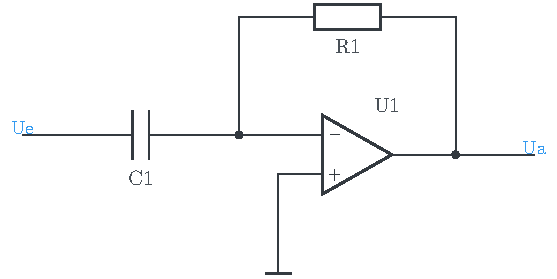
\includegraphics[width=0.618\textwidth]{circuits/differenzier.pdf}
  \end{center}
  \caption{Differentiatorschaltung}
\end{figure}

\begin{gather*}
i_{R_1} = - i_{C_1}\\
\frac{u_a}{R_1} = - C_1 \cdot \frac{\dif u_e}{\dif t}
\end{gather*}
\eqbox{
u_a = - {R_1 C_1} \cdot \frac{\dif u_e}{\dif t}
}{0.382\textwidth}
Der Differentiator differenziert die Eingangsspannung, wichtet das Ergebnis mit
$RC$ und invertiert es.


\subsection{Frequenzverhalten}
Das Frequenzverhalten des Bipolartransistors wird durch die
Sperrschichtkapazität $C_{BC}$, welche im Normalbetrieb dominiert, sowie die
Diffusionskapazität $C_{BE}$ bestimmt, da diese im Ersatzschaltbild
frequenzabhängige Widerstände darstellen. 

\subsection{Grenzfrequenz und Bandbreite}
\begin{figure}[H]
  \begin{center}
    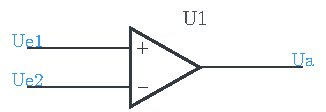
\includegraphics[width=0.618\textwidth]{circuits/komparator.pdf}
  \end{center}
  \caption{Einfache Komparatorschaltung}
\end{figure}

\[ U_a = V_0 (U_p - U_n) = V_0 (U_{e1} - U_{e2})\]

Ist $U_{e1}$ größer als $U_{e2}$ gerät der Operationsverstärker an seine
maximale positive Ausgangsspannung (idealerweise die
Versorgungsspannung), ist $U_{e1}$ kleiner als $U_{e2}$ an die maximal negative.
Legt man $U_{e2}$ auf einen konstanten positiven Referenzspannungswert, so verschiebt sich
die Kennline aus Abbildung 1 nach rechts.

\begin{figure}[H]
  \begin{center}
    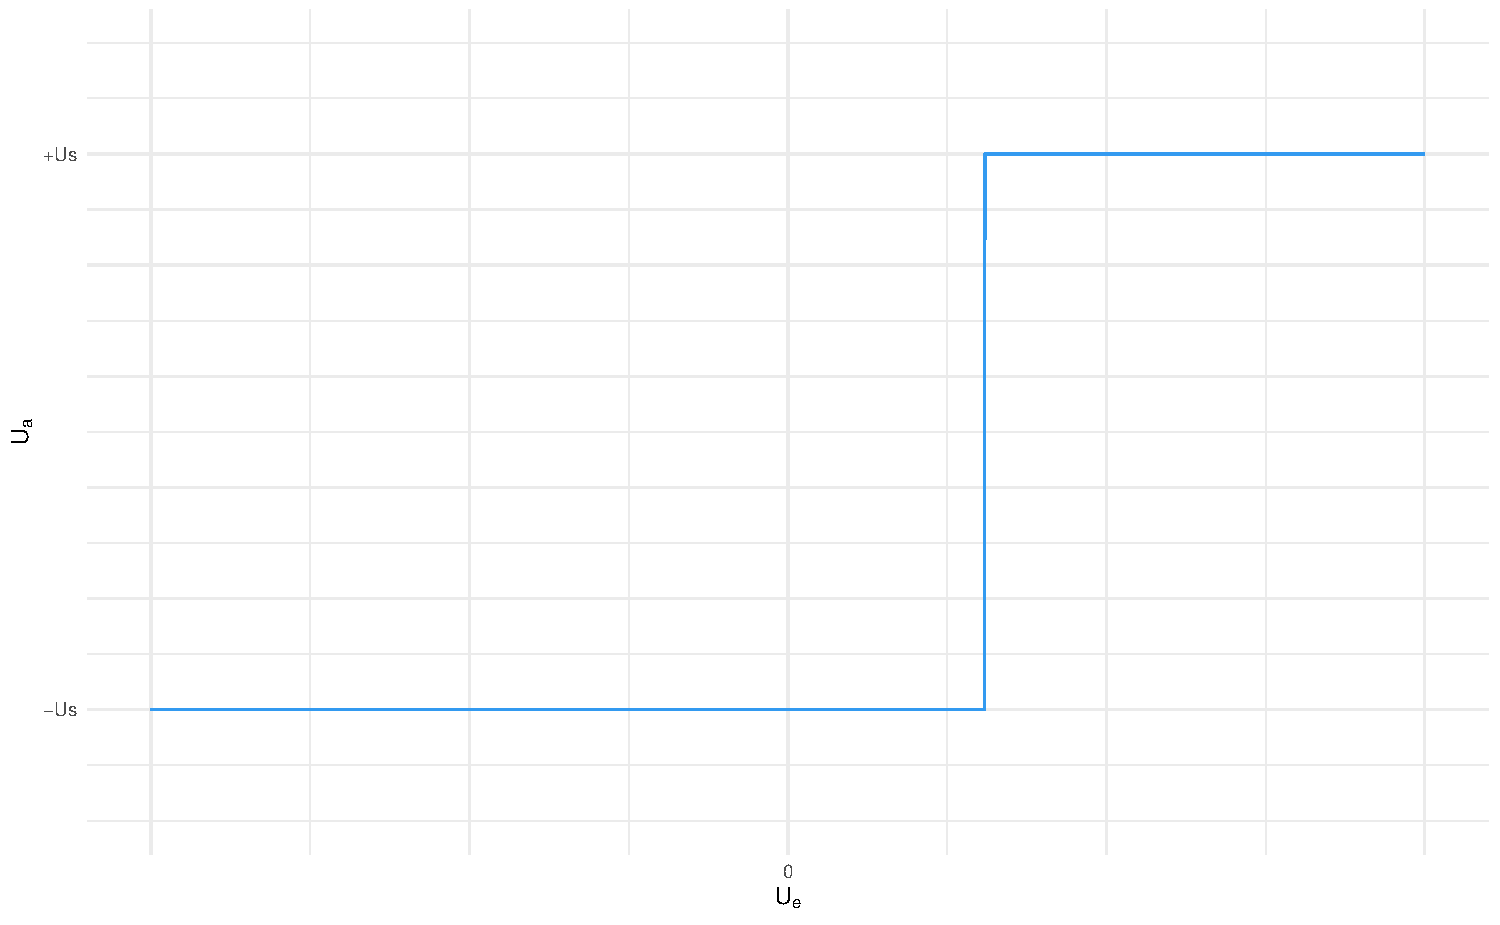
\includegraphics[width=\textwidth]{1_11/comparator.pdf}
  \end{center}
  \caption{Übertragungskennlinie der Komparatorschaltung mit positiver Referenzspannung ($U_{e2}$)}
\end{figure}


Zwischen invertierendem und nichtinvertierendem Eingang des
Operationsverstärkers können zwei Dioden antiparallel geschaltet werden, um die
Eingangsdifferenzspannung auf $\pm 0.7 \, \si{\volt}$ zu begrenzen. Zusätzlich
müssen dann zur Strombegrenzung Widerstände vor die Eingangs-/ Referenzspannung
geschaltet werden. 

\subsection{Millertheorem}
\begin{figure}[H]
  \begin{center}
    \includegraphics[width=\textwidth]{circuits/schmitt.pdf}
  \end{center}
  \caption{Schmitt-Trigger-Schaltung}
\end{figure}

\subsection{Grenzfrequenz der Emitterschaltung}
\begin{figure}[H]
  \begin{center}
    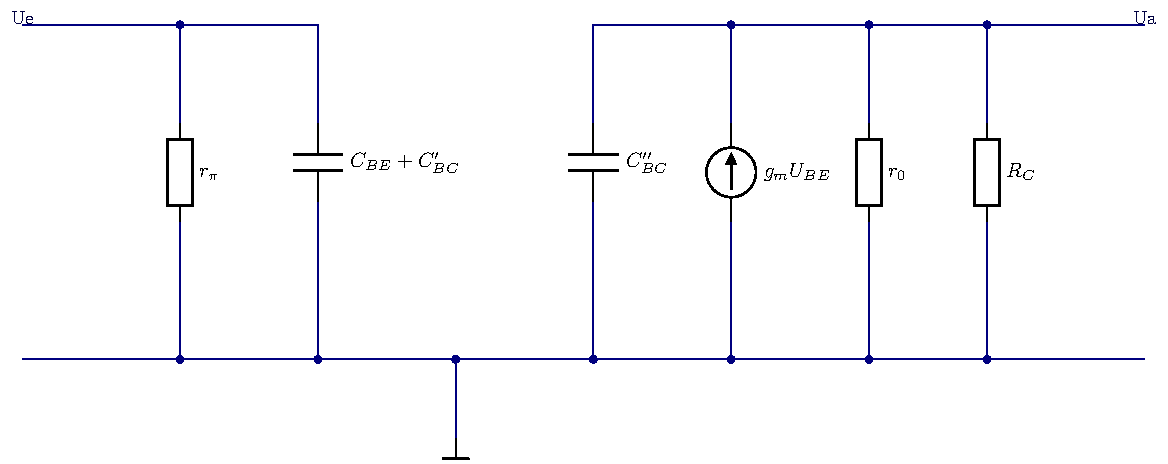
\includegraphics[width=0.618\textwidth]{circuits/commonEmitter_freq.pdf}
  \end{center}
  \caption{ESB der Emitterschaltung mit Millerkapazitäten}
\end{figure}

Die obere Grenzfrequenz der Schaltung wird durch die parasitären Kapazitäten des
Bipolartransistors bestimmt, die untere durch die Koppelkondensatoren der Schaltung

Eingangskreis:
\[0 = \frac{U_1}{r_\pi} + U_1 j \omega (C'_{BC}+C_{BE})-I_b\]

\noindent Ausgangskreis:
\[0 = g_m U_1 + \frac{U_a}{r_0 // R_C} - U_a j \omega C_{BC}''\]

\noindent Übertragungsfunktion
\[\frac{U_a}{U_e} = \frac{\frac{1}{r_\pi} +
    j\omega(C_{BC}'+C_{BE}) -g_m}{\frac{1}{r_0 // R_C} - j\omega C_{BC}''}\]

\noindent Grenzfrequenz
\[\omega_{gr} = \frac{1}{(C_{BE}+C_{BC}')r_\pi }\]

\[\left( \omega_{gr} = \frac{1}{(C_{BC}' + C_{BE})\cdot \frac{1}{g_m} - r_0
      C_{BC}''} \right) ? \]

% 2
%%%%%%%%%%%%%%%%%%%%%%%%%%%%%%%%%%%%%
  
\includepdf{./titlepage/titlepage2.pdf}
  \clearpage
  \setcounter{page}{1}
%%%%%%%%%%%%%%%%%%%%%%%%%%%%%%%%%%%%%

\section{Versuchsaufgaben} 

\setcounter{subsection}{1}
\subsection{Arbeitspunktbestimmung}
Die Ströme und Spannungen konnten teilweise nur indirekt gemessen werden und
mussten daher aus mehreren Messungen berechnet werden.

\subsubsection{ES\_IGK1}
Der Kollektorstrom $I_C$ der Schaltung wurde durch die Messung der Spannung über dem
Widerstand $R_3$ ($V_2 - U_C$)und entsprechender Division durch dessen Widerstandswert
ermittelt.
\[I_C  = \frac{V_2 - U_c}{R_3} = \frac{12.01 \, \si{\volt} - 6.38 \,
    \si{\volt}}{1.3 \, \si{\kilo\ohm}} = 4.33 \, \si{\milli\ampere}\]

Die Kollektorspannung konnte dann über Messung des Emitterpotentials $U_E$ gegen Masse
und Differenzbildung mit dem vorher bestimmten Wert $U_c$ bestimmt werden.
\[U_{CE} = U_C - U_E = 6.38 \, \si{\volt} - 0.436 \, \si{\volt} = 5.944 \, \si{\volt}\]

Der Basisstrom ist die Differenz aus dem Strom durch $R_1$ und dem Strom durch
$R_2$.
\[I_B = \frac{V_2 - U_B}{R_1}-\frac{U_B}{R_2} = \frac{12 \, \si{\volt} - 1.149
    \, \si{\volt}}{43 \, \si{\kilo\ohm}} - \frac{1.149 \, \si{\volt}}{5.1 \,
    \si{\kilo\ohm}} = 27.58 \, \si{\micro\ampere}\]

Die statische Stromverstärkung ist damit
\[B = \frac{I_C}{I_B} = \frac{4.33 \, \si{\milli\ampere}}{27.58 \,
    \si{micro\ampere}} = 157\]

Aus dem Datenblatt des 2N3904 Bipolartransistors lässt sich bei einem
Kollektorstrom vom etwa $I_C = 4 \, \si{\milli\ampere}$ und einer
Kollektor-Emitter-Spannung von $U_{CE} = 10 \, \si{\volt}$ ein
Stromverstärkungsfaktor von $B = 150$ ablesen. (Datenblatt onsemi Abb. 11).

\begin{figure}[H]
  \begin{center}
    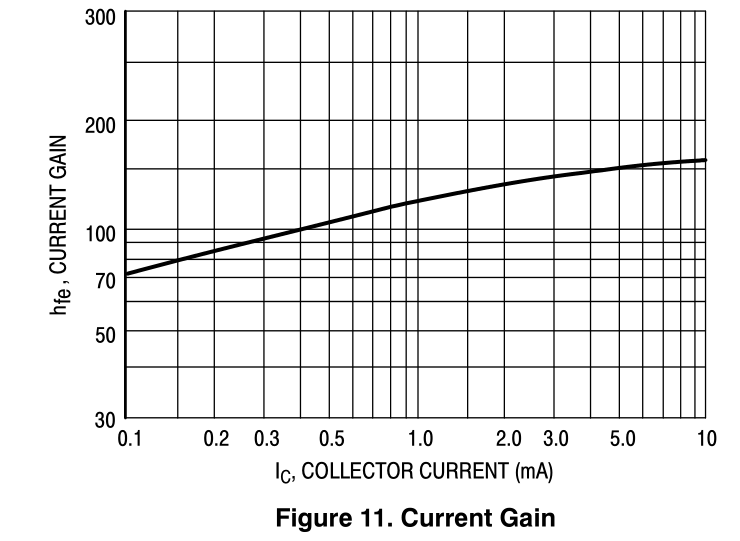
\includegraphics[width=0.618\textwidth]{2_2/ds1}
  \end{center}
  \caption{Quelle: http://onsemi.com}
\end{figure}

\subsubsection{ES\_IUGK1}
Die Arbeitspunktwerte der zweiten und dritten Schaltung wurden entsprechend 2.2.1 bestimmt.

\begin{table}[H]
\begin{center}
\begin{tabular}{c | c}
  $U_C$ & $6.06 \, \si{\volt}$\\
  \hline
  $U_E$ & $0.53 \, \si{\volt}$\\
  \hline
  $U_B$ & $1.23 \, \si{\volt}$\\
\end{tabular}
\end{center}
\caption{Zwischenwerte der Schaltung ES\_IUGK1}
\end{table}

\begin{table}[H]
\begin{center}
\begin{tabular}{c | c}
  $I_C$ & $5.23 \, \si{\milli\ampere}$\\
  \hline
  $U_{CE}$ & $5.53 \, \si{\volt}$\\
  \hline
  $I_{B}$ & $24.15 \, \si{\micro\ampere}$\\
  \hline
  $B$ & $216 $\\
\end{tabular}
\caption{Arbeitspunktwerte der Schaltung ES\_IUGK1}
\end{center}
\end{table}

\subsubsection{KS\_BOS1}

\begin{table}[H]
\begin{center}
\begin{tabular}{c | c}
  $U_C$ & $12.01 \, \si{\volt}$\\
  \hline
  $U_E$ & $4.37 \, \si{\volt}$\\
  \hline
  $U_B$ & $5 \, \si{\volt}$\\
  \hline
  $U_{R1}$ & $6.9 \, \si{\volt}$\\
  \hline
  $U_{R3}$ & $0.63 \, \si{\volt}$\\
\end{tabular}
\end{center}
\caption{Zwischenwerte der Schaltung KS\_BOS1}
\end{table}

\begin{table}[H]
\begin{center}
\begin{tabular}{c | c}
  $I_C$ & $ 1.45 \, \si{\milli\ampere}$\\
  \hline
  $U_{CE}$ & $ 7.91 \, \si{\volt}$\\
  \hline
  $I_{B}$ & $ 4.26 \, \si{\micro\ampere}$\\
  \hline
  $B$ & $340.38$\\
\end{tabular}
\caption{Arbeitspunktwerte der Schaltung KS\_BOS1}
\end{center}
\end{table}



\subsection{Emitterschaltung mit Stromgegenkopplung: ES\_IGK1}
\subsubsection{Spannungsverstärkung}
Die Werte zur Bestimmung der Spannungsverstärkungen wurden bei einer
Eingangsspannung von $U_{\mathrm{RMS}} = 5 \, \si{\milli\volt}$ und einer
Frequenz von $f_e = 1 \, \si{\kilo\hertz}$ bestimmt. Der Lastwiderstand wurde
von $100 \, \si{\kilo\ohm}$ bis $1 \, \si{\kilo\ohm}$ variiert. Die
Spannungsverstärkungen bei den jeweiligen Lastwiderstandswerten ist dann
der Quotient aus Ausgangs- und Eingangsspannung. Die Spannungswerte wurden
als RMS-Werte am Oszilloskop gemessen. Der interne Lastwiderstand beträgt $R_{\mathrm{L,intern}} =
100 \, \si{\kilo\ohm}$.

\begin{table}[H]
  \begin{center}
    \begin{tabular}{|c|c|c|c|}
      \hline
      $U_e / \si{\milli\volt}$ & $U_a / \si{\milli\volt}$ & $R_{\mathrm{L,gesamt}} / \si{\kilo\ohm}$ & $V_u$\\
      \hline
      \hline

      4.99 & 810.96 & 100 & 162.5\\
      4.97 & 790.5 & 33.33 & 159.1\\
      4.98 & 721.6 & 9.09 & 144.90\\
      4.97 & 363.9 & 0.99 & 73.22\\
      \hline
    \end{tabular}

  \end{center}

  \caption{RMS-Spannungswerte und daraus resultierende Verstärkung bei
    verscheidenen Lastwiderständen}

\end{table}

\begin{figure}[H]
  \begin{center}
    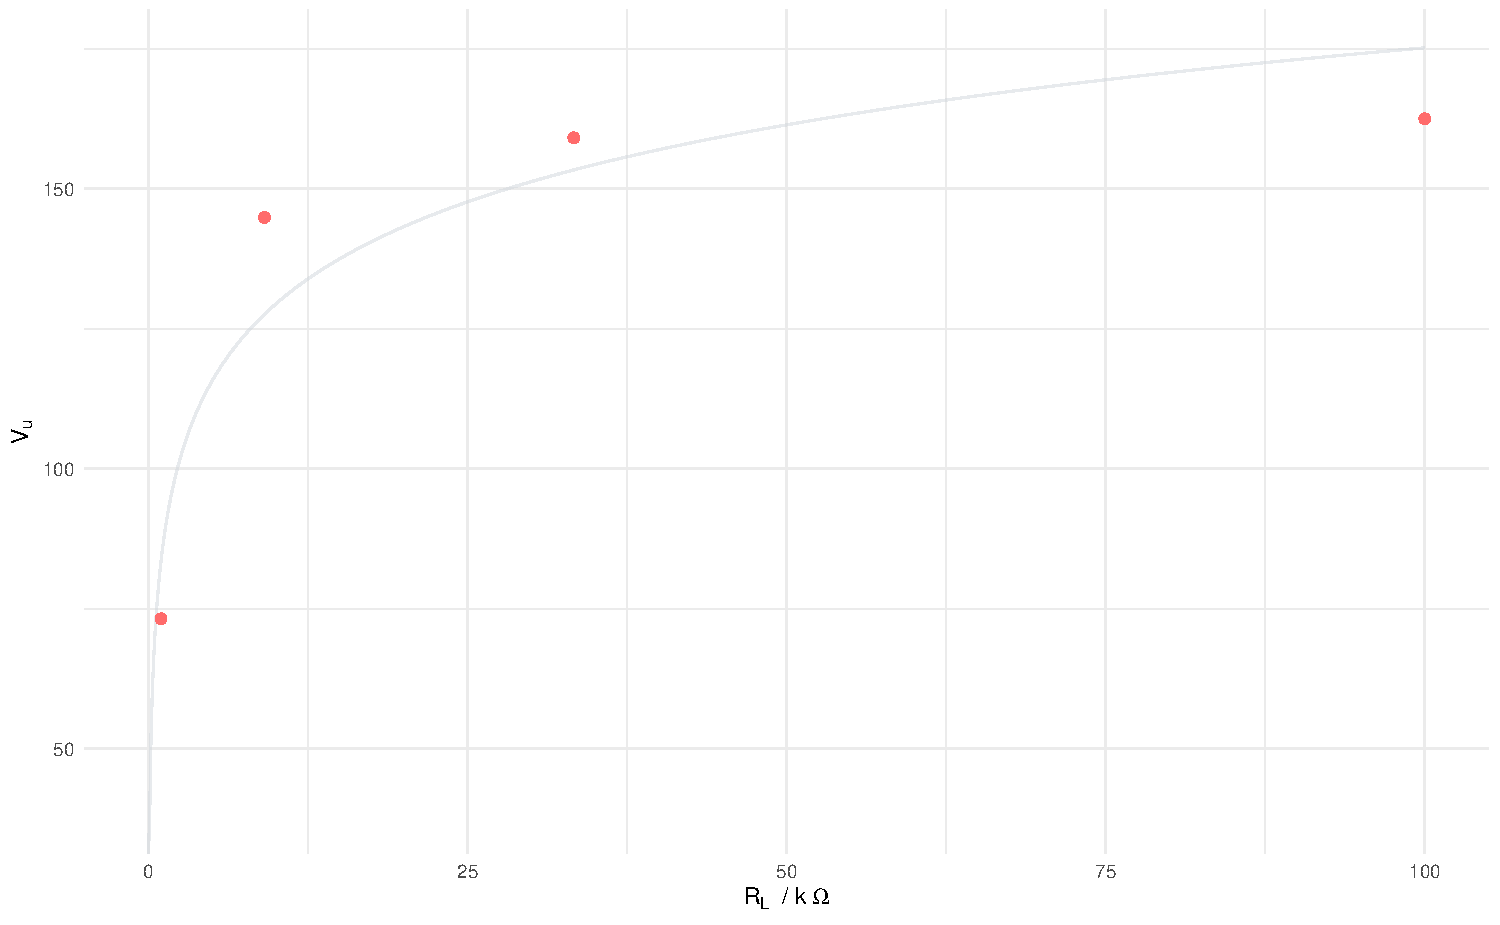
\includegraphics[width=\textwidth]{2_3/2_3_1.pdf}
  \end{center}
  \caption{Graph der Messwerte}
\end{figure}

Der Anstieg des Graphen entspricht der Steilheit $g_m$ des Transistors. Die
Steilheit im Arbeitspunkt ist etwa
\[g_m = \frac{I_C}{U_T} = \frac{4.33 \, \si{\milli\ampere}}{26 \,
    \si{\milli\volt}} = 166.53 \, \si{\milli\siemens}\]

Der theoretische Zusammenhang ist
\[V_u = - g_m \cdot R_L \] 

Der scheinbar lineare Zusammenhang ist aus dem Messwertgraphen jedoch nicht
erkennbar. Dies liegt daran, dass der interne Kollektorwiderstand $R_3$ als
Parallelschaltung in den Gesamtlastwiderstand eingeht.
\[V_u = -g_m \cdot R_3 // R_{\mathrm{L,extern}}\]

$R_3 = 1.3 \, \si{\kilo\ohm}$ legt hier durch die Parallelschaltung den
theoretischen Grenzwert der Spannungsverstärkung fest. \[|V_{u,max}| = 188.26 \,
  \si{\milli\siemens} \cdot 1.3 \, \si{\kilo\ohm} \approx 245\]


Bei hohen externen Widerstandswerten dominiert der Widerstand $R_3$ in der
Parallelschaltung, wodurch der Gesamtlastwiderstand etwa $R_3$ ist, die
Verstärkung läuft gegen einen konstanten Wert.
Bei geringen Widerstandswerten muss die Parallelschaltung berücksichtigt
werden.

Durch Berücksichtung des Kollektorwiderstandes erhält man dann den erwarteten Zusammenhang.

\begin{figure}[H]
  \begin{center}
    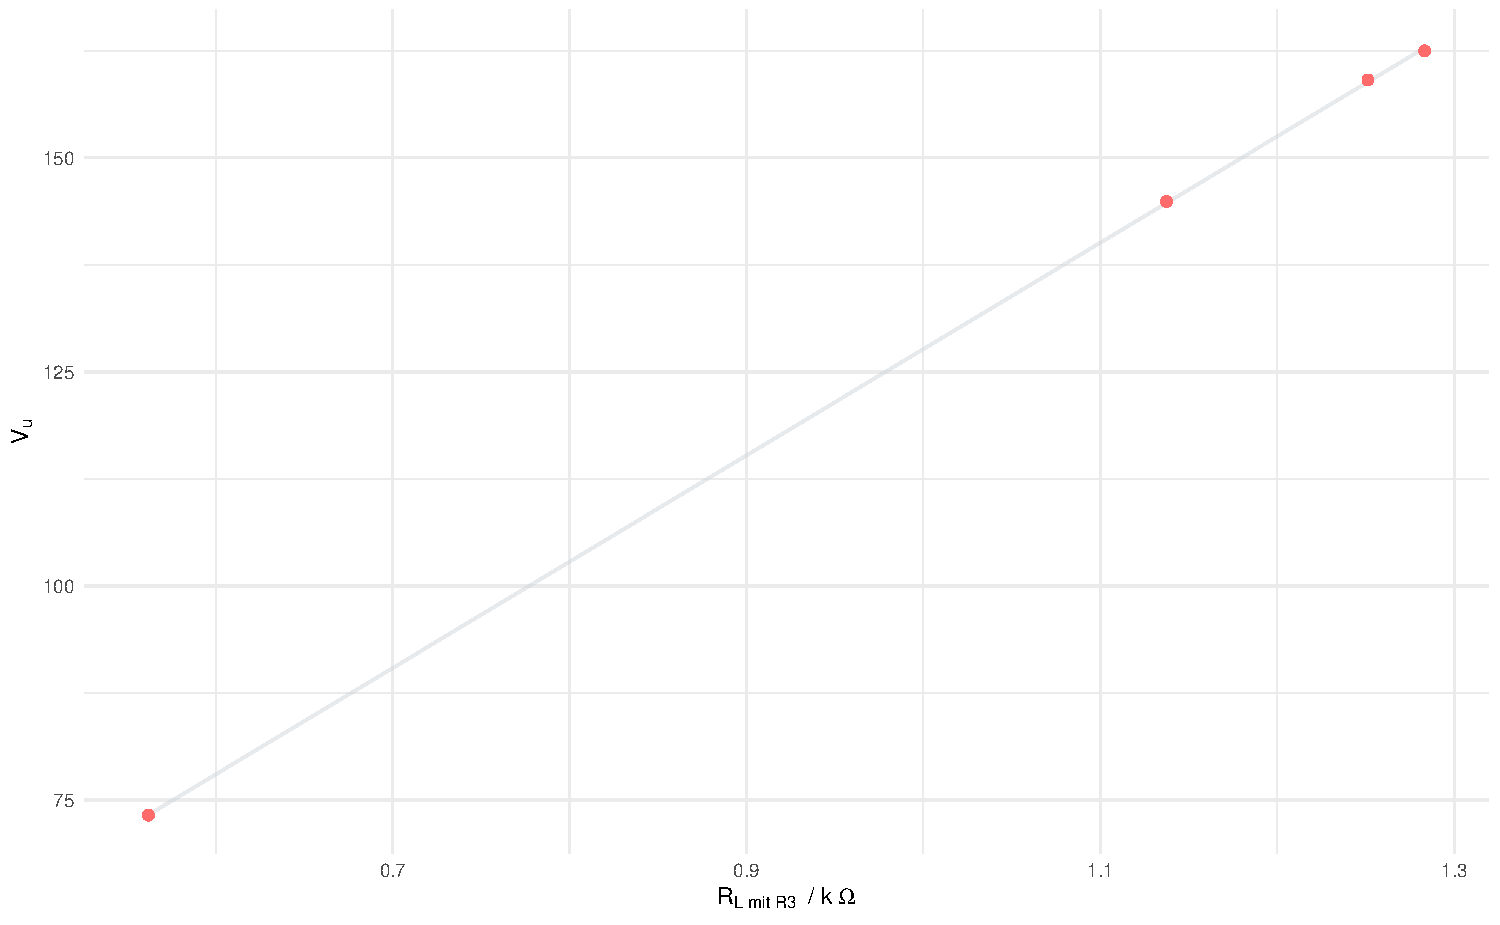
\includegraphics[width=\textwidth]{2_3/2_3_1_corrected.pdf}
  \end{center}
  \caption{Graph der Messwerte, korrigiert}
\end{figure}

Die resultierende Steilheit ist somit:
\[g_m \approx 128 \, \si{\milli\siemens}\]


(Da die Eingangsspannung den Kollektorstrom jedoch etwas verschiebt, ist die
Steilheit nicht konstant, was zu einer Abweichung des theoretisch linearen
Verhaltens führt. Außerdem wurde der Ausgangswiderstand des Transistors nicht berücksichtigt)

\subsubsection{Eingangswiderstand}
Mithilfe der U/2-Methode wurde der Eingangswiderstand der Schaltung bei
konstantem Lastwiderstand von $100 \, \si{\kilo\ohm}$ (kein externer Widerstand)
und einer Frequenz von $1 \, \si{\kilo\hertz}$ bestimmt.

\[U_{a1} = \frac{U_a}{2} = 413 \, \si{\milli\volt}\]

Der dabei ermittelte Eingangswiderstand ist
\[r_e = 800 \, \si{\ohm}\]

\begin{figure}[H]
  \begin{center}
    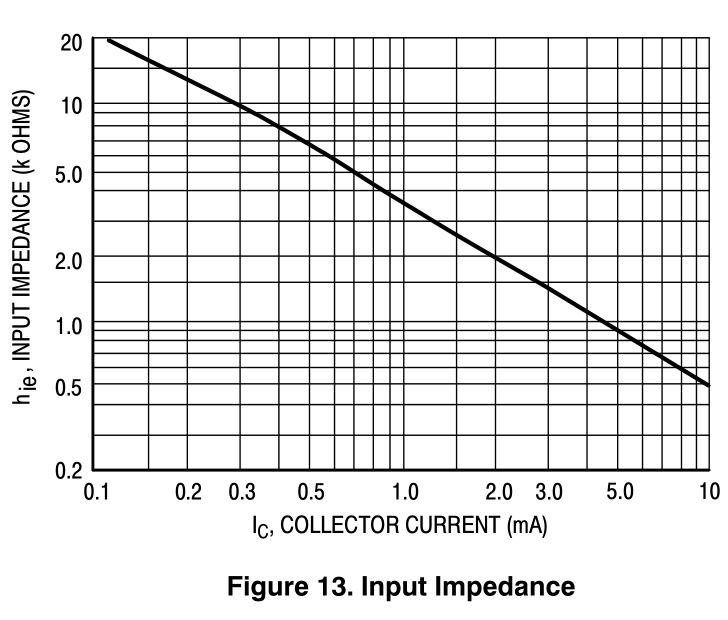
\includegraphics[width=0.618\textwidth]{inputimp}
  \end{center}
  \caption{Quelle: http://onsemi.com}
\end{figure}

Aus dem Transistordatenblatt Abb. 13 ist bei einem Kollektorstrom von $I_C = 4.33 \,
\si{\milli\ampere}$ ein $r_\pi$ von etwa $1 \, \si{\kilo\ohm}$ ablesbar. Der
theoretische Eingangswiderstand der Emitterschaltung ist
\[r_{e,\mathrm{theoretisch}} = R_1 // R_2 // r_\pi \approx 820 \,\si{\ohm}\]

Der messtechnisch ermittelte Wert stimmt also ziemlich genau mit dem
theoretischen überein. Mögliche Abweichungen entstehen durch ungenaue
Widerstandswerte, Messabweichungen/Fehlerfortpflanzung und ungenaues Ablesen von
Werten aus Datenblattkurven.

\subsubsection{Ausgangswiderstand}
Der Ausgangswiderstand bestimmt sich über die umgestellte Spannungsteilerformel
am Ausgangskreis. $U_{a0}$ ist die Leerlaufspannung, ohne Belastung. $U_{a1}$
die Ausgangsspannung bei Belastung mit dem externen Widerstand $R_L = 10 \, \si{\kilo\ohm}$.
\[U_{a1} = U_{a0} \cdot \frac{R_L}{r_a + R_L}\]
\[r_a = R_L \left( \frac{U_{a0}}{U_{a1}} -1 \right)\]

\[U_{a0} = 821.45 \, \si{\milli\volt}\]
\[U_{a1} = 731.50 \, \si{\milli\volt}\]

\[r_a = 10 \, \si{\kilo\ohm} \left( 821.45 \frac{ \, \si{\milli\volt}}{731.50 \,
      \si{\milli\volt}} -1 \right) = 1.2297 \, \si{\kilo\ohm}\]

\begin{figure}[H]
  \begin{center}
    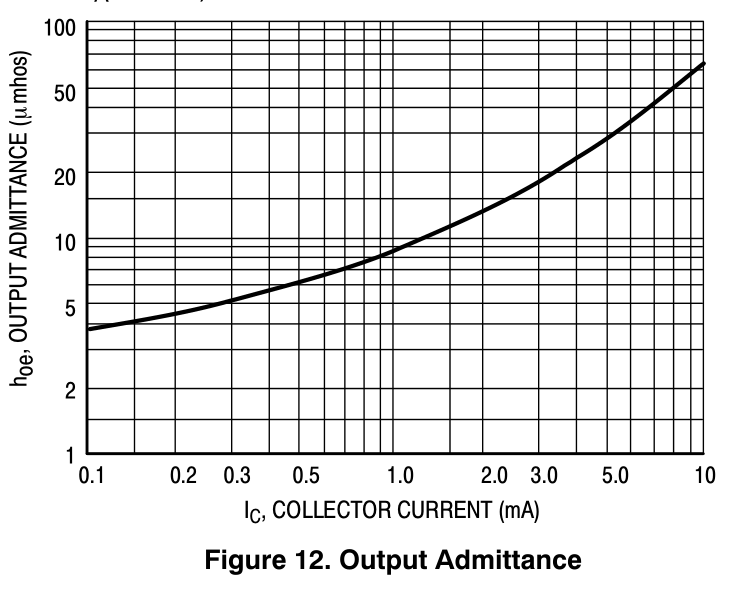
\includegraphics[width=0.618\textwidth]{outadmittance}
  \end{center}
  \caption{Quelle: http://onsemi.com}
\end{figure}

Der theoretische Ausgangswiderstandswert ergibt sich mit den Datenblattwerten zu
\[r_a = R_3 // R_L // r_0 = 1.3 \, \si{\kilo\ohm} // 100 \, \si{\kilo\ohm}// \, 33.33 \si{\kilo\ohm} \approx 1.236 \, \si{\kilo\ohm}\]

Der messtechnisch ermittelte Wert stimmt erneut gut mit dem theoretischen überein.

\subsubsection{Amplituden-Frequenzgang}
Der Amplituden-Frequenzgang wurde durch das Durchlaufen der
Eingangsspannungsfrequenzen von $0$ bis $10 \, \si{\kilo\hertz}$ und die Messung
der Ausgangsspannungswerte (RMS) bei einer Eingangsspannung von $U_e =
5\,\si{\milli\volt}_{\mathrm{RMS}}$ ermittelt.

\begin{figure}[H]
  \begin{center}
    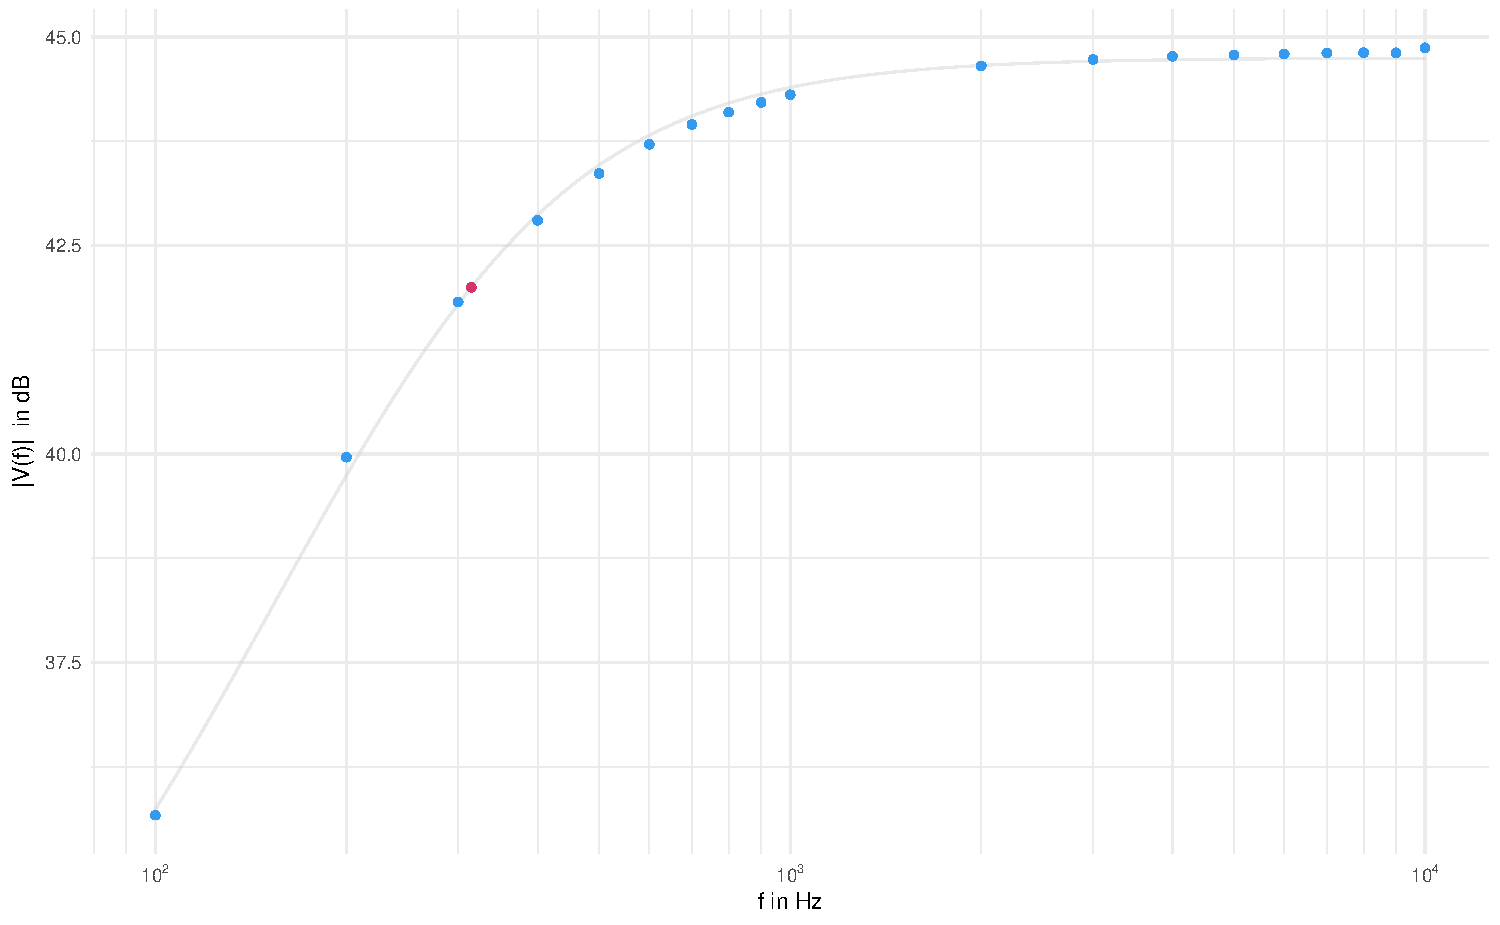
\includegraphics[width=\textwidth]{2_3/2_3_frequenzgang.pdf}
  \end{center}
  \caption{Amplitudenfrequenzgang der Messung}
\end{figure}

Die durch Regression ermittelte Grenzfrequenz ist
\[f_g \approx 300 \, \si{\hertz}\]

Vor der Grenzfrequenz steigt die Verstärkung mit etwa $25 \, \si{\deci\bel}$ pro
Dekade. Weit hinter der Grenzfrequenz nimmt sie den entsprechenden Wert aus
2.3.1 an.

$C_E$ ($C_3$) stellt wechselstromseitig einen Kurzschluss dar, wodurch der
Emitterwiderstand diesbezüglich wegfällt und die Verstärkung für 
Wechselspannungen deren Frequenz hoch genug ist nicht beeinflusst. Bei
niedrigeren Frequenzen ist die Reaktanz des Kondensators jedoch nicht
ausreichend gering, um den Einfluss von $R_E$ vollständig zu beseitigen, weshalb
die Verstärkung in diesem Fall sinkt.

\begin{table}[H]
\begin{center}
\begin{tabular}{@{}cc@{}}
\toprule
$f / \, \si{\hertz}$ & $u_\mathrm{a} / \, \si{\milli\volt}$ \\ \midrule
  \midrule
100                  & 303.7                       \\
200                  & 497.8                       \\
300                  & 616.8                       \\
400                  & 690.3                       \\
500                  & 736.5                       \\
600                  & 766.7                       \\
700                  & 787.9                       \\
800                  & 801.5                       \\
900                  & 812.38                      \\
1000                 & 820.96                      \\
2000                 & 854.3                       \\
3000                 & 862                         \\
4000                 & 865.7                       \\
5000                 & 867.5                       \\
6000                 & 868.6                       \\
7000                 & 869.6                       \\
8000                 & 870                         \\
9000                 & 870                         \\
10000                & 876                         \\ \bottomrule
\end{tabular}
\end{center}
\caption{Messwerte des Frequenzganges}
\end{table}

\subsection{Emitterschaltung mit Parallelgegenkopplung: ES\_IUGK1}
\subsubsection{Spannungsverstärkung}
Die Werte zur Bestimmung der Spannungsverstärkungen wurden bei einer
Eingangsspannung von $U_{\mathrm{RMS}} = 100 \, \si{\milli\volt}$ und einer
Frequenz von $f_e = 1 \, \si{\kilo\hertz}$ bestimmt. Der Lastwiderstand wurde
von $100 \, \si{\kilo\ohm}$ bis $1 \, \si{\kilo\ohm}$ variiert. Die
Spannungsverstärkungen bei den jeweiligen Lastwiderstandswerten ist dann
der Quotient aus Ausgangs- und Eingangsspannung. Die Spannungswerte wurden
als RMS-Werte am Oszilloskop gemessen. Der interne Lastwiderstand beträgt $R_{\mathrm{L,intern}} =
100 \, \si{\kilo\ohm}$.


\begin{table}[H]
  \begin{center}
    \begin{tabular}{|c|c|c|c|}
      \hline
      $U_e / \si{\milli\volt}$ & $U_a / \si{\milli\volt}$ & $R_{\mathrm{L,gesamt}} / \si{\kilo\ohm}$ & $V_u$\\
      \hline
      \hline
      99.92 & 1080 & 100 & 10.81\\
      99.95 & 1050 & 33.33 & 10.51\\
      99.93 & 954.5 & 9.09 & 9.55\\
      99.99 & 475.4 & 0.99 & 4.76\\
      \hline
    \end{tabular}
  \end{center}
  \caption{RMS-Spannungswerte und daraus resultierende Verstärkung bei
    verscheidenen Lastwiderständen (ohne $R_3$)}
\end{table}

\begin{figure}[H]
  \begin{center}
    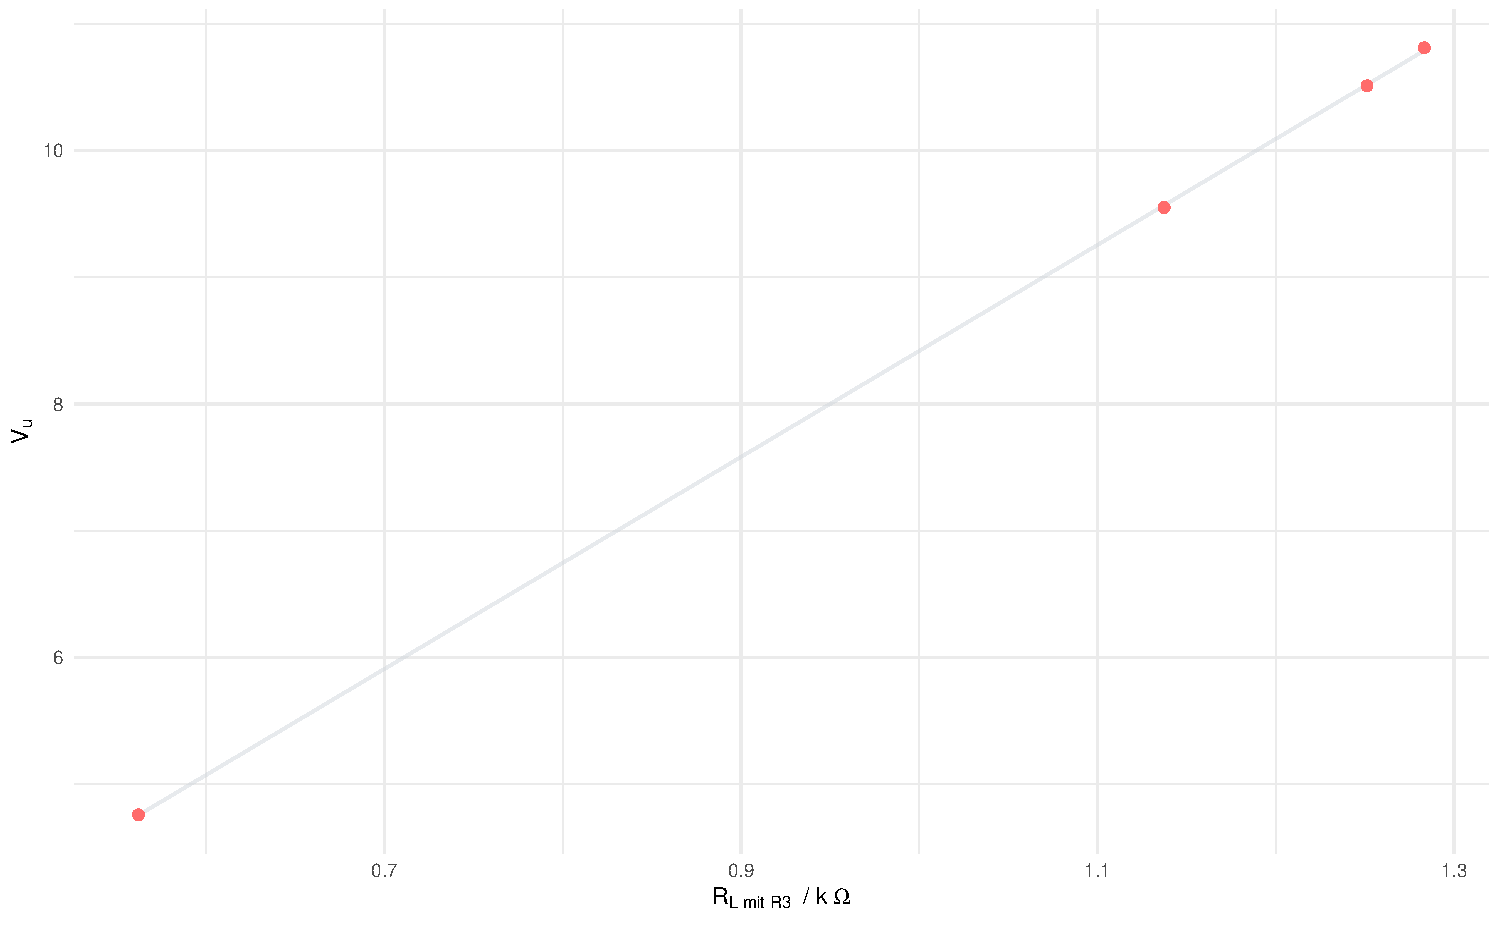
\includegraphics[width=\textwidth]{2_4/2_4_1_R3.pdf}
  \end{center}
  \caption{Graph der Messwerte, $R_3$ berücksichtigt}
\end{figure}

Der Zusammenhang zwischen Lastwiderstand und Verstärkung ist dem der vorherigen
Schaltung (ESIGK1) ähnlich. Die theoretische Steilheit des Transistors im Arbeitspunkt ist hier
\[g_{m,\mathrm{theoretisch}} = \frac{I_C}{U_T} = \frac{5.23 \, \si{\milli\ampere}}{26 \,
    \si{\milli\volt}} = 201.154 \, \si{\milli\siemens}\]

Durch die Gegenkopplung der Ausgangs- auf die Eingangsspannung wird, wie der
Versuch bestätigt, die Verstärkung der Emitterschaltung deutlich verringert.

\subsubsection{Eingangswiderstand}
Der Eingangswiderstand wurde auch hier nach der $U/2$-Methode bestimmt.

$U_{a0} = 1.08 \, \si{\volt}$
$U_{a1} = 500 \, \si{\milli\volt}$

Der dabei ermittelte Widerstandswert ist
\[r_e = 11 \, \si{\kilo\ohm}\]

Aus dem Datenblatt:
\[r_\pi = 0.9 \, \si{\kilo\ohm}\]
\[r_0 = 33.33 \, \si{\kilo\ohm}\]

Der theoretische Widerstandswert ist
\[r_{e} = R_2 // ((1+B_N) \cdot (R_5 // r_0) + r_\pi) = 21.35 \, \si{\kilo\ohm}\]

Der theoretische Wert ist etwa das Doppelte des theoretischen Wertes,
möglicherweise ist ein Rechen- oder Messfehler aufgetreten.

\subsubsection{Ausgangswiderstand}
Der Ausgangswiderstand wurde wie in 2.3.3 aus Messung zweier Spannungswerte
ermittelt. Der externe Ausgangslastwiderstand ist $R_L = 10 \, \si{\kilo\ohm}$

\[U_{a0} = 1080 \,\si{\milli\volt}\]
\[U_{a1} =  954.5 \,\si{\milli\volt}\]

\[r_a = 10 \, \si{\kilo\ohm} \left( \frac{1080 \, \si{\milli\volt}}{954.5 \,
      \si{\milli\volt}} -1 \right) \approx 1.3 \, \si{\kilo\ohm}\]





\subsection{Kollektorschaltung mit Bootstrap: KS\_BOS1}
\subsubsection{Spannungsverstärkungen}
Die Werte zur Bestimmung der Spannungsverstärkungen wurden bei einer
Eingangsspannung von $U_{\mathrm{RMS}} = 1 \, \si{\volt}$ und einer
Frequenz von $f_e = 1 \, \si{\kilo\hertz}$ bestimmt. Der Lastwiderstand wurde
von $100 \, \si{\kilo\ohm}$ bis $1 \, \si{\kilo\ohm}$ variiert. Der interne Lastwiderstand beträgt $R_{\mathrm{L,intern}} =
100 \, \si{\kilo\ohm}$.


\begin{table}[H]
  \begin{center}
    \begin{tabular}{|c|c|c|c|}
      \hline
      $U_e / \si{\milli\volt}$ & $U_a / \si{\milli\volt}$ & $R_{\mathrm{L,gesamt}} / \si{\kilo\ohm}$ & $V_u$\\
      \hline
      \hline
      997.7 & 995 & 100 & 0.9973\\
      1020 & 994 & 33.33 & 0.9745\\
      1020 & 992 & 9.09 & 0.9726\\
      1000 & 918 & 0.99 & 0.918\\
      \hline
    \end{tabular}
  \end{center}
  \caption{RMS-Spannungswerte und daraus resultierende Verstärkung bei
    verscheidenen Lastwiderständen}
\end{table}

Die Messung am Oszilloskop war sehr verrauscht, weshalb sich unter Umständen
starke Abweichungen ergeben können.

\begin{figure}[H]
  \begin{center}
    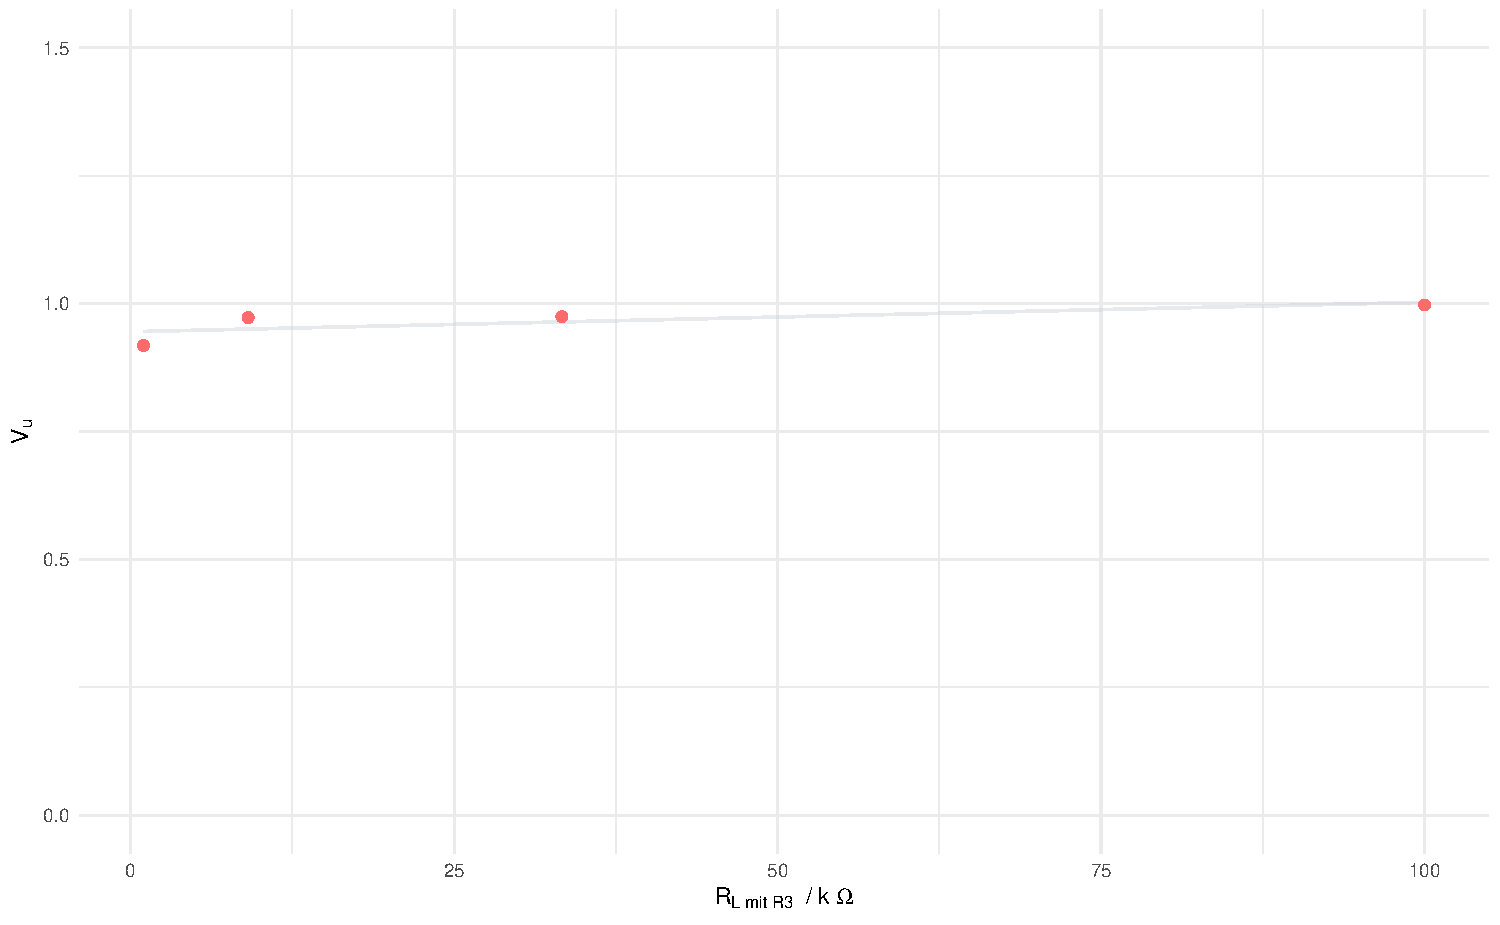
\includegraphics[width=\textwidth]{2_5/2_5_1.pdf}
  \end{center}
  \caption{Graph der Messwerte}
\end{figure}

Es lässt sich gut erkennen, dass die Verstärkereigenschaft der
Kollektorschaltung ($V_u \approx 1$) erfüllt ist.

\subsubsection{Eingangswiderstand}
Der theoretische Wert des Eingangswiderstandes der Kollektorschaltung ohne
Bootstrap, d.h. wenn $R_3 = 0$ und C weggelassen wird,  ist ( mit $B = 294$ im Arbeitspunkt)
\[r_{e,\mathrm{noBT}} = R_1 // R_2 // (B \cdot (R_4 // R_5)) = 184.5 \,\si{\kilo\ohm}\]

Messtechnisch konnte der Eingangsreihenwiderstand für die U/2 Methode nicht auf
einen ausreichend hohen Wert gestellt werden, da die verwendetete
Widerstandsdekade dies nicht hergab.

\subsubsection{Ausgangswiderstand}
Wie in den vorherigen Aufgaben ist der Ausgangswiderstand (bei einem
Lastwiderstand von $10 \, \si{\kilo\ohm}$)

\[r_a = R_L \left( \frac{U_{a0}}{U_{a1}} -1 \right)\]
\[r_a = 10 \, \si{\kilo\ohm} \left( \frac{995 \, \si{\milli\volt}}{993 \,
      \si{\milli\volt}} -1 \right)= 30.24 \, \si{\milli\ohm}\]

Der Ausgangswiderstand der Kollektorschaltung ohne Bootstrap, mit den gleichen
restlichen Widerstandswerten, ($I_C = 1.299 \, \si{\milli\ampere}$ (LTSPICE)) ist
\[r_a \approx \frac{1}{g_m} = \frac{U_T}{I_C} = \frac{26 \,
    \si{\milli\volt}}{1.299 \, \si{\milli\ampere}} = 20.02 \, \si{\ohm}\]

\subsection{Vergleich der Grundschaltungen}
\begin{table}[H]
\centering
\caption{Qualitativer Vergleich der Grundschaltungen mit Beispielwerten}
\label{my-label}
\begin{tabular}{|*{4}{p{0.25\textwidth}|}}
\hline
Schaltung     & Emitterschaltung & Kollektorschaltung & Basisschaltung \\ \hline
  \hline
Spannungsverstärkung   &    hoch      & $\approx< 1$            & hoch (wie Emitterschaltung) \\ \hline
Eingangswiderstand &   durchschnittlich ($\approx 1 \, \si{\kilo\ohm}$)       &  am höchsten ($\approx 100 \, \si{\kilo\ohm}$)           &      gering $\approx 50 \, \si{\ohm}$      \\ \hline
Ausgangswiderstand  &  durchschnittlich $\approx 50 \, \si{\kilo\ohm}$        &            gering $\approx 200 \,\si{\ohm}$&  sehr hoch $\approx 1 \, \si{\mega\ohm} $       \\ \hline
Bsp. Einsatzgebiet        &      allg. Verstärkerschaltung    &   Impedanzwandler         &    Hochfrequenzverstärker (hohe Grenzfrequenz)        \\ \hline
\end{tabular}
\end{table}

\end{document}
